%%%%%%%%%%%%%%%%%%%%%%% file template.tex %%%%%%%%%%%%%%%%%%%%%%%%%
%
% This is a general template file for the LaTeX package SVJour3
% for Springer journals.          Springer Heidelberg 2010/09/16
%
% Copy it to a new file with a new name and use it as the basis
% for your article. Delete % signs as needed.
%
% This template includes a few options for different layouts and
% content for various journals. Please consult a previous issue of
% your journal as needed.
%
%%%%%%%%%%%%%%%%%%%%%%%%%%%%%%%%%%%%%%%%%%%%%%%%%%%%%%%%%%%%%%%%%%%
%
% First comes an example EPS file -- just ignore it and
% proceed on the \documentclass[•]{•} line
% your LaTeX will extract the file if required
\begin{filecontents*}{example.eps}
%!PS-Adobe-3.0 EPSF-3.0
%%BoundingBox: 19 19 221 221
%%CreationDate: Mon Sep 29 1997
%%Creator: programmed by hand (JK)
%%EndComments
gsave
newpath
  20 20 moveto
  20 220 lineto
  220 220 lineto
  220 20 lineto
closepath
2 setlinewidth
gsave
  .4 setgray fill
grestore
stroke
grestore
\end{filecontents*}
%
\RequirePackage{fix-cm}
%
%\documentclass{svjour3}                     % onecolumn (standard format)
%\documentclass[smallcondensed]{svjour3}     % onecolumn (ditto)
\documentclass[smallextended]{svjour3}       % onecolumn (second format)
%\documentclass[twocolumn]{svjour3}          % twocolumn
%
\smartqed  % flush right qed marks, e.g. at end of proof
%
% \usepackage{mathptmx}      % use Times fonts if available on your TeX system
%
% insert here the call for the packages your document requires
\usepackage{latexsym}
\usepackage{graphicx}
\usepackage{amsmath, amssymb, amsfonts, mathtools}
\usepackage{enumerate}
\usepackage{algorithm, algpseudocode}
\usepackage{txfonts, pxfonts}
\usepackage{grffile}
\usepackage{caption, subcaption}
\usepackage{listings}
\usepackage[table, xcdraw]{xcolor}
\usepackage{rotating}
\usepackage{multirow}
\usepackage{chronology}
\usetikzlibrary{arrows, shapes}
\usepackage{tabularx}
\usepackage{hyperref}
\usepackage{libertine}
\usepackage{pgfgantt}
\usepackage{lscape}
\usepackage{enumitem}

\usepackage{tikz} % drawing graph
\usetikzlibrary{arrows.meta} % drawing graph
%\usepackage[tight,footnotesize]{subfigure}

\input amssym.def
\input amssym.tex
%
% please place your own definitions here and don't use \def but
\newcommand{\mmlcpt}{$mbMML_{CPT}$ }
\newcommand{\mbptmml}{$MBPT_{mml}$ }
\DeclareMathOperator*{\argmin}{arg\,min}
\DeclarePairedDelimiter\floor{\lfloor}{\rfloor}
\newcommand{\ci}{\mathrel{\text{\scalebox{1.07}{$\perp\mkern-10mu\perp$}}}}
\newcommand{\independent}{\perp\mkern-9.5mu\perp}
\newcommand{\notindependent}{\centernot{\independent}}
\newcommand{\qedwhite}{\hfill \ensuremath{\Box}}
\algnewcommand\algorithmicforeach{\textbf{for each}}
\algdef{S}[FOR]{ForEach}[1]{\algorithmicforeach\ #1\ \algorithmicdo}

\makeatletter
% Taken from http://ctan.org/pkg/centernot
\newcommand*{\centernot}{%
  \mathpalette\@centernot
}
\def\@centernot#1#2{%
  \mathrel{%
    \rlap{%
      \settowidth\dimen@{$\m@th#1{#2}$}%
      \kern.5\dimen@
      \settowidth\dimen@{$\m@th#1=$}%
      \kern-.5\dimen@
      $\m@th#1\not$%
    }%
    {#2}%
  }%
}
\makeatother

%
% Insert the name of "your journal" with
% \journalname{myjournal}
%
% This file can be modified and used in other conferences as long
% as credit to the authors and supporting agencies is retained, this notice
% is not changed, and further modification or reuse is not restricted.

\begin{document}

\title{Weak recursively simplicial graphs
%On checking Markov blankets consistency with DAGs via graph immoralization%\thanks{Grants or other notes
%about the article that should go on the front page should be
%placed here. General acknowledgments should be placed at the end of the article.}
}
%\subtitle{Do you have a subtitle?\\ If so, write it here}

%\titlerunning{Short form of title}        % if too long for running head

\author{First Author         \and
        Second Author \and
        Third Author
}

%\authorrunning{Short form of author list} % if too long for running head

\institute{F. Author \at
              first address \\
              Tel.: +123-45-678910\\
              Fax: +123-45-678910\\
              \email{fauthor@example.com}           %  \\
%             \emph{Present address:} of F. Author  %  if needed
           \and
           S. Author \at
              second address
}

\date{Received: date / Accepted: date}
% The correct dates will be entered by the editor

\maketitle

\section{The complexity of checking Markov blankets consistency with DAGs via morality}

\section{Introduction}
Introduced by (peral citation) as the smallest subset of variables in a Bayesian network, given which the target variable is conditional independent from the rest of the variables, Markov blanket has became popular for scaling up learning Bayesian network structures and causal discovery (give a few citations). It naturally divides the problem of learning a global structure into learning local structures within Markov blankets that can be done in parallel. Markov blankets have also been applied during data preprocessing as a feature selection technique that looks for the smallest but most informative subset of features for predicting a target, to reduce computational complexity of having a large set of features (citation). In a faithful Bayesian network (citation), the Markov blanket of a target variable consists of its parents, children and children's other parents (a.k.a., spouses) (Figure \ref{fg:mb_example}).  
\begin{figure}[H]
\centering
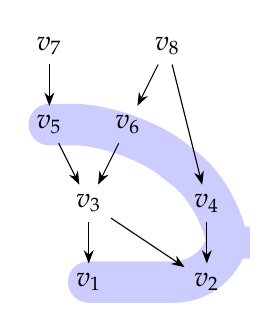
\begin{tikzpicture}
\begin{scope}[>={Stealth[black]},              
              every edge/.style={draw=black}]
    \node (A) at (0.5,0) {$v_1$};
    \node (B) at (2,0) {$v_2$};
    \node (C) at (0.5,1) {$v_3$};
    \node (D) at (2,1) {$v_4$};
    \node (E) at (0,2) {$v_5$};
    \node (F) at (1,2) {$v_6$};
    \node (G) at (0,3) {$v_7$};    
    \node (H) at (1.5,3) {$v_8$};   
    \path [->] (G) edge (E);
    \path [->] (H) edge (F);
    \path [->] (H) edge (D);
    \path [->] (E) edge (C);
    \path [->] (F) edge (C);
    \path [->] (C) edge (A);
    \path [->] (C) edge (B);
    \path [->] (D) edge (B);
\end{scope}
% Highlight the A_1 -> B_1 -> C_2 path. Use layers to draw
% behind everything.
\begin{pgfonlayer}{background}
	\draw[rounded corners=2em,line width=1.5em,blue!20,cap=round]
		(A.center) -- (B.east) -- (D.east) -- (F.center) -- (E.center);
\end{pgfonlayer}
\end{tikzpicture}
\caption{A DAG, in which the Markov blanket of $v_3$ is $\{v_5,v_6,v_1,v_2,v_4\}$.}
\label{fg:mb_example}
\end{figure}
Since 19xx, researchers have been developing efficient algorithms for learning Markov blankets from observational data (many citations). Due to the complexity of the problem, most of these learners are heuristics based on either statistical significant tests or objective functions for optimally balancing between predictive power and complexity. A set of subsets of variables $B=\{B_1, \dots, B_n\}$, one for each variable $v_i \in V$, which are learned from a Markov blanket learner must satisfy the symmetric and consistent properties for $B$ being a valid set of Markov blankets. The symmetric property is a direct consequence of the graphical interpretation of Markov blankets in a directed acyclic graph (DAG). That is, $v_i \in B_j$ if and only if $v_j \in B_i$. The consistent property entails that there exists at least one DAG $G=(V,E)$ s.t. the set of parents, children and spouses of node $v_i \in V$ equals $B_i$ for all $v_i$ in $G$. 

Outputs of Markov blanket learners are generally used without explicitly knowing the role of each member in $B_i$ relative to the target variable $v_i$. This does not stop the symmetric property to be checked (and possibly enforced), but makes it non-trivial for checking their consistency (with a DAG). Without being consistent, a set of learned Markov blankets could lead to inconsistent local structures within Markov blankets, which has to be resolved at some stage during the transition from local to global structure learning. In this paper, we drew a connection between Markov blankets' consistency and graph morality, and presented algorithms for checking morality for undirected graphs with various of maximum degrees. The contribution of this paper is threefold. First, we introduced the concepts of \textit{weak recursively simplicial} and \textit{perfect elimination kit} to help checking morality and prove important proerties of moral graphs that will be studied in future investigation. Second, we developed polynomial time algorithms for checking morality for maximum degree $3$ and $4$ graphs. And we proved that checking morality for graphs with maximum degree $5$ and above is NP-complete. Third, all the algorithms for checking morality, including a backtracking algorithm for graphs with maximum degree $5$ and above, give a way of \textit{immoralizing} moral graphs to obtain DAGs. 


\section{Preliminary}
In this section, we introduced the concepts that will be used throughout this paper. 

\begin{definition}
\label{def:graph}
A \textbf{graph} is a pair $G = (V, E)$ comprising a set $V$ of vertices (or nodes) together with a set $E$ of edges (or arcs).
\end{definition}
The vertex and edge set of $G$ is denoted by $V(G)$ and $E(G)$ respectively. Throughout this paper, we use $u,v$ to represent vertices in $V$ and $uv$ to represent an (undirected) edge in $E$. A graph is generally referring to an undirected graph, unless it is said otherwise. 

\begin{definition}
\label{def:digraph}
A \textbf{directed graph} is a graph $G=(V,E)$, where $E$ is a set of ordered pairs of distinct vertices in $V$.
\end{definition}

\begin{definition}
\label{def:dag}
A directed graph $G = (V, E)$ is called a \textbf{directed acyclic graph} if it contains no directed cycles. 
\end{definition}
In a directed acyclic graph $G=(V,E)$, $u$ is a \textit{parent} of $v$, denoted by $u \in P(v)$ (or $v$ is a \textit{child} of $u$), if there is a directed edge from $u$ to $v$. $u$ is an \textit{ancestor} of $v$ (or $v$ is a \textit{descendent} of $u$) if there is a directed path from $u$ to $v$. $v$ is a \textit{nondescendent} of $u$ if $v$ is not a descendent of $u$.

Bayesian network structures are often represented by directed acyclic graphs (a.k.a., DAGs), because acyclic ensures no variable is a cause of itself if the Bayesian networks model causality. 
\begin{definition}
\label{def:markov}
Let $\mathcal{P}$ be a joint probability distribution of the random variables in $V$, and $G=(V,E)$ be a directed acyclic graph. We say $<G, \mathcal{P}>$ satisfies the \textbf{Markov condition} if for every variable $v_i \in V$, it is conditionally independent of its non-descendants  given its parents set.
\end{definition}

\begin{definition}
\label{def:bn}
Let $\mathcal{P}$ be a joint probability distribution of the random variables in $V$, and $G=(V,E)$ be a directed acyclic graph. We say $<G, \mathcal{P}>$ forms a \textbf{Bayesian network} if it satisfies the Markov condition. 
\end{definition}

\begin{definition}
\label{def:mb}
Let $<G=(V,E),\mathcal{P}>$ be a Bayesian network. The \textbf{Markov blanket} of $u$ in the Bayesian network, denoted by $B(u)$, is the minimum subset of variables s.t. 
\begin{align*}
u \!\perp\!\!\!\perp_{\mathcal{P}} V\setminus B[u] \mid B(u),
\end{align*}
where $B[u]=B(u)\cup \{u\}$.
\end{definition}

\begin{definition}
\label{def:hybrid_g}
A \textbf{hybrid graph} is a graph consisting of directed and undirected edges. 
\end{definition}

\begin{definition}
\label{def:skeleton}
The \textbf{skeleton} of a hybrid graph is the undirected graph obtained by dropping directions of all directed edges. 
\end{definition} 

\begin{definition}
\label{def:moral_g}
The \textbf{moral graph} of a directed acyclic graph $G=(V,E)$ is the skeleton of the hybrid graph $H=(V,E\cup F)$, where $F=\{uv \mid u,v \in P_G(x) \text{ and } \{uv,vu\} \cap E=\emptyset\}$.
\end{definition}
The obove definition implicitly states a way of obtaining a moral graph from a DAG. That is, by joining all pairs of non-adjacent parents in the DAG, then dropping all the directions. The process is obtaining a moral graph from a DAG is also known as \textit{moralization} (Figure \ref{fg:envelope}). 
\begin{figure}[H]
\centering
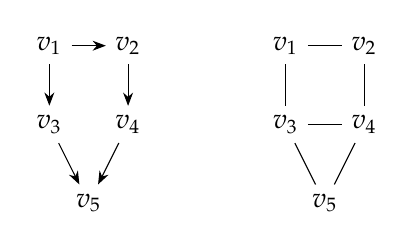
\begin{tikzpicture}
%\tikzstyle{place}=[circle,draw=blue!50,fill=blue!20,thick,inner sep=0pt,minimum size=6mm]
\begin{scope}
    \node (A) at (0,0) {$v_1$};
    \node (B) at (1,0) {$v_2$};
    \node (C) at (0,-1) {$v_3$};
    \node (D) at (1,-1) {$v_4$};
    \node (E) at (0.5,-2) {$v_5$};
    
    \node (F) at (3,0) {$v_1$};
    \node (G) at (4,0) {$v_2$};
    \node (H) at (3,-1) {$v_3$};
    \node (I) at (4,-1) {$v_4$};
    \node (J) at (3.5,-2) {$v_5$};
\end{scope}

\begin{scope}[>={Stealth[black]},
              every node/.style={fill=white,circle},
              every edge/.style={draw=black}]
    \path [->] (A) edge (B);
    \path [->] (A) edge (C);
    \path [->] (B) edge (D);
    \path [->] (C) edge (E);
    \path [->] (D) edge (E);
    
    \path [-] (F) edge (G);
    \path [-] (F) edge (H);
    \path [-] (G) edge (I);
    \path [-] (H) edge (I);
    \path [-] (H) edge (J);
    \path [-] (I) edge (J);
%    \path [-] (B) edge [bend right=60] (E); 
\end{scope}
\end{tikzpicture}
\caption{A DAG $G$ and its moral graph $H$.}
\label{fg:envelope}
\end{figure}
If a given Bayesian network $<G,\mathcal{G}>$ is faithful, the Markov blanket of a variable $u$ consists of its parents and children which are directly connected to $u$ and its spouses which are connected to $u$ via its children. For any spouse $v$ of $u$ that is neither a parent nor child of $u$, the edge $uv$ will be added to the moral graph of $G$ via moralization. Therefore, the Markov blanket of a node in a faithful Bayesian network has an one-to-one correspondance to the neighbourhood of the node in the Bayesian network's moral graph. For example, in Figure \ref{fg:envelope} $B_G(v_3)=\{v_1,v_5,v_4\}=N_H(v_3)$.
\begin{definition}
\label{def:collider}
A \textbf{collider} in a hybrid graph is a node with at least two parents. 
\end{definition}

\begin{definition}
\label{def:consistent_ext}
A directed acyclic graph $G$ is a \textbf{consistent extension} of a hybrid graph $H$ if $G$ and $H$ have the same skeleton and colliders. 
\end{definition}

\begin{definition}
\label{def:subgraph}
Let $G=(V,E)$ and $G'=(V',E')$ be two graphs. If $V \subseteq V'$ and $E \subseteq E'$, then $G$ is a \textbf{subgraph} of $G'$, written as $G \subseteq G$. 
\end{definition}

\begin{definition}
\label{def:induced_subgraph}
Let $G=(V,E)$ and $G'=(V',E')$ be two graphs. If $G\subseteq G'$ and $uv \in E'$ for all $u,v \in V$, then $G$ is an \textbf{induced subgraph} of $G'$, written as $G=G'[V]$.
\end{definition}
For simplicity purposes, if $U\subset V$ then we use $G-U$ to denote $G[V\setminus U]$. If $U=\{u\}$, then we use $G-u$. If $U=V(H)$, then we use $G-H$. Similarly, if $F\subset E$ then we use $G+E$ and $G-F$ to denote $(V,E\cup F)$  and $(V,E\setminus F)$ respectively. If $E = \{uv\}$ then we use $G+uv$ or $G-uv$ instead.

\begin{definition}
Let $G=(V,E)$ be a graph. The set of \textbf{neighbours} of $u$ in $G$ is $N(u)=\{v \in V \mid uv \in E\}$. The closed neighbourhood of $u$ in $G$ is $N[u]=N(u)\cup \{u\}$.
\end{definition}

\begin{definition}
Let $G=(V,E)$ be a graph. The \textbf{maximum degree} of the graph $\Delta(G)=\max\{d(u) \mid u \in V\}$, where $d(u)=|N(u)|$ is the degree of $u$.
\end{definition}

\begin{definition}
A \textbf{clique} is a subset of nodes in a graph where every two distinct nodes are adjacent. 
\end{definition}

\begin{definition}
A \textbf{simplicial node} in a graph is a node whose neighbours form a clique. 
\end{definition}

\begin{definition}
Let $G=(V,E)$ be a graph. The \textbf{deficiency} of a node $x$ in $G$ is $D(x)=\{uv \mid u, v \in N(x) \text{ and } uv \notin E\}$.
\end{definition}
A node $u$ is a simplicial in $G$ if and only if $D(u)=\emptyset$. That is, no edge needs to be filled in to make the neighbours of $u$ a clique. We write $D(G)\neq \emptyset$ if $D_G(u)\neq \emptyset, \forall u \in V$. And $D(G)=\emptyset$ if $\exists x \in V$ s.t. $D_G(x)=\emptyset$.

\begin{definition}
An \textbf{m-cycle} in a graph is a sequence of nodes $\{v_1, \dots, v_{m+1}\}$ where $v_1 = v_{m+1}$ and all the other nodes are distinct.  
\end{definition}

\begin{definition}
A graph is \textbf{chordal} if each $m$-cycle for $m \ge 4$ has a chord.
\end{definition}

\begin{definition}
A graph $G=(V,E)$ is \textbf{recursively simplicial} if it contains a simplicial node $u$ and the induced subgraph $G-u$ is recursively simplicial. 
\end{definition}

\begin{definition}
\label{def:wrs}
A graph $G=(V,E)$ is \textbf{weak recursively simplicial} if $\exists x \in V$ with $D_G(x)=\emptyset$ and $\exists E'\subseteq \{uv \in E \mid u,v \in N_G(x)\}$ s.t. the subgraph $G'=G-x-E'$ is weak recursively simplicial. 
\end{definition}
If a graph is recursively simplicial (i.e., chordal), it is also weak recursively simplicial with $E'=\emptyset$ for each simplicial node $x$. The converse, however, is not true. For example, the moral graph in Figure \ref{fg:envelope} is weak recursively simplicial, but it is not chordal. 

\begin{definition}
An \textbf{ordering} of a graph $G=(V,E)$ with $n$ vertices is a bijection $\alpha: \{1, \dots, n\} \leftrightarrow V$. 
\end{definition}

\begin{definition}
A set of \textbf{excesses} of a graph $G=(V,E)$ according to an ordering $\alpha$ is a bijection $\epsilon_{\alpha}: \alpha \leftrightarrow \{\epsilon_{\alpha}(v_1), \dots, \epsilon_{\alpha}(v_n)\}$, where $\epsilon_{\alpha}(v_i) \subseteq E(G[N(v_i)])$ consists of some edges between the neighbours of $v_i$.
\end{definition}
The composition $\kappa=(\alpha,\epsilon_{\alpha})$ of an ordering and a set of excesses is called an elimination kit of a graph $G$. For example, an ordering $\alpha=(v_5,v_3,v_4,v_1,v_2)$ and a set of excess $\epsilon_{\alpha}=(\emptyset,\emptyset,\emptyset,\emptyset,\emptyset)$ form an elimination kit of the moral graph in Figure \ref{fg:envelope}. We use $\kappa(1)$ to denote the node $\alpha(1)$ and its excess $\epsilon_{\alpha}(\alpha(1))$. By using the concept of elimination kit, we can define a subgraph $G^i=G-\{\kappa(1),\dots,\kappa(i-1)\} \subset G$. 

\begin{definition}
Let $G=(V,E)$ be a graph and $\kappa=(\alpha, \epsilon_{\alpha})$ be an elimination kit of $G$. It is a \textbf{perfect elimination kit} if $D_{G^i}(v)=\emptyset$ for each node $v$ with $\alpha^{-1}(v)=i$.
\end{definition}
The elimination kit mentioned above is not perfect, because $D_{G^2}(v_3)\neq \emptyset$. The only perfect elimination kit (pek) for the moral graph in Figure \ref{fg:envelope} $\alpha=(v_5,v_3,v_4,v_1,v_2)$ and $\epsilon_{\alpha}=(\{v_3v_4\},\emptyset,\emptyset,\emptyset,\emptyset)$. In general, a graph may have none, one or more than one pek. 

\iffalse
The following are some well-known properties of chordal graphs (citation!!!).
\begin{proposition}
\label{prop:chordal_properties}
The following properties of an undirected graph $F$ are equivalent:
\begin{enumerate}
\item $F$ is chordal. 
\item $F$ is recursively simplicial. 
\item $F$ can be oriented into a DAG $G$ s.t. the moral graph of $G$ is $F$.
\item $F$ can be oriented into a DAG $G$ s.t. $F$ and $G$ imply the same conditional independencies. 
\end{enumerate}
\end{proposition}
As a consequence of 1 and 4, $F$ can be oriented into a DAG $G$ s.t. $B_X^F = B_X^G$. The following proposition states that there  exists non-chordal graphs, who can be oriented into DAGs with the same Markov blanket families. 

\begin{proposition}
Let $\mathcal{F}$ be the set of chordal graphs $F=(V,E)$ and $\mathcal{B}$ be the set of Markov blanket families of DAGs over $V$. Then there exists an injective but non-surjective function $\phi: \mathcal{F} \rightarrow \mathcal{B}$. 
\end{proposition}
\begin{proof}
Let $F_1, F_2$ be two identical chordal graphs. It implies $B_V^{F_1} = B_V^{F_2}$. Since $F_i$ is a chordal, it can be oriented into a DAG $G_i$ s.t. $B_V^{F_i} = B_V^{G_i}, \forall i \in \{1,2\}$. It follows that $B_V^{G_1}=B_V^{G_2}$, so $\phi$ is an injective function. 

For any given DAG $G$, it has a unique moral graph $F$ s.t. $B_V^G=B_V^F$. Figure \ref{fg:wrs_non_chordal} is an example of a DAG and its moral graph, which is non-choral. Hence, $\phi$ is non-surjective. \qed
\end{proof}
\fi

\section{Weak recursively simplicial graphs}
The first main task of this section is to prove there is a one-to-one correspondance between moral graphs and weak recursively simplicial graphs. To do this, we prove the following two lemmas. 

\begin{lemma}
\label{lm:moral_implies_wrs}
Let $G=(V,E)$ be a DAG and $H$ be the moral graph of $G$. Then $H$ is weak recursively simplicial. 
\end{lemma}

\begin{proof}
The lemma is proved by induction on the number of nodes. Let $G(n)$ and $H(n)$ denote a DAG and its moral graph over a set of $n$ nodes. The lemma is true for $n \le 3$, because all graphs contain three nodes or less are WRS. Assuming $H(n)$ is WRS for an arbitrary $n \ge 4$. We want to show that the moral graph $H(n+1)$ is also WRS. It is known that each DAG contains at least one sink $x$, and $x$ becomes a simplicial node in the DAG's moral graph because its parents form a clique after moralization. Hence, the moral graph $H(n+1)$ contains a simplicial node $x$. By removing $x$ and the edges that were introduced by moralization to make $x$'s neighbourns a clique, the resulting graph $H(n)$ is the moral graph of the DAG $G(n)$ obtained by removing $x$ from $G(n+1)$. The inductive hypothesis assumes that each moral graph $H(n)$ is WRS. Hence, $H(n+1)$ is also WRS. \qed
\end{proof}
Lemma \ref{lm:moral_implies_wrs} suggests that the moral graph of any DAG is WRS. To prove there is a one-to-one correspondance it is remaining to show that the converse is also true. That is, a WRS graph is the moral graph of a DAG. 

\begin{lemma}
\label{lm:wrs_implies_moral}
Let $H=(V,E)$ be a weak recursively simplicial graph. Then $H$ is the moral graph of a DAG. 
\end{lemma}

\begin{proof}
The lemma is proved by induction on the number of nodes $n$. The statement is true for $n=1$, because a single node graph $H(1)$ is both the moral graph of $G(1)$ and a WRS graph. Assuming the lemma is true for an arbitrary $n\ge 2$. That is, any WRS graph $H(n)$ with $n\ge 2$ is the moral graph of a DAG $G(n)$. Each WRS graph has a simplicial node. Assuming $x$ is a simplicial node of a WRS graph $H(n+1)$ and $x$ is the first in the ordering $\alpha$ (i.e., $\alpha^{-1}(x)=1$). When orienting $H(n+1)$, we first let all the edges connect to $x$ be directed towards it. Furthermore, some edges between the neighbours of $x$ are removed so that the resulting graph $H(n)$ is still WRS. By the inductive assumption, $H(n)$ is the moral graph of a $G(n)$. Hence, by attaching $x$ and the edges connect to it onto $G(n)$ we obtain a DAG $G(n+1)$, whose moral graph is $H(n+1)$. \qed
\end{proof}

\begin{theorem}
\label{thm:wrs_equal_moral}
A graph is weak recursively simplicial if and only if it is the moral graph of a DAG. 
\end{theorem}
\begin{proof}
The theorem follows from the Lemma \ref{lm:moral_implies_wrs} and Lemma \ref{lm:wrs_implies_moral}. \qed
\end{proof}
Moralization from a DAG to an undirected graph is trivial, whilst orienting a moral graph to obtain a DAG with the same Markov blankets is not trivial. We call such a process \textit{immoralization}. It is beyond the focus of this paper but is an interesting topic that worth further investigating. It has a potential to get from a (symmetric and consistent) set of Markov blankets to a DAG that may not likely to be the generating Bayesian network structure, but could be used as an initial structure for structure learning and causal discovery. 

Chodality is considered to be a \textit{hereditary} property of a graph, because the subgraph is still chordal after removing a simplicial node from a chordal graph. Similarly, morality is also a hereditary property, but in the sense that the subgraph is still moral after removing a simplicial node and some edges between its neighbours from a moral graph. 

\iffalse
% this result is not difficult, but doesn't fit the content of this paper. 
\begin{corollary}
Let $\mathcal{F}=\{F=(V,E) \mid F \text{ is weak recursively simplicial}\}$ be the set of weak recursively simplicial graphs over $V$ and $\mathcal{B} = \{B_V^G \mid \text{for all DAG $G$ over $V$}\}$ be the set of Markov blanket families of any DAG over $V$. Then $|\mathcal{F}| = |\mathcal{B}|$. 
\end{corollary}
\begin{proof}
It is straightforward that there is a one-to-one correspondance between $\mathcal{B}$ and moral graphs. Hence, Corollary \ref{cor:wrs_equal_moral} implies that $\mathcal{F}$ has a one-to-one correspondance with $\mathcal{B}$, so equal cardinality. \qed
\end{proof}
\fi

Next, we present a backtracking algorithm for checking whether or not a given graph $G=(V,E)$ is WRS. If it is, the algorithm will return TRUE and orient it into a hybrid graph that always has a consistent DAG extension \cite{dor1992simple}, whose Markov blankets are identical to $G$'s.
\begin{algorithm}[]
\caption{Checking morality using backtracking}
\label{alg:wrs_bktr}
\begin{algorithmic}[]
	\Require{a graph $G=(V,E)$}
	
    \Function{$\phi$}{$F$}
    \If{$G=\emptyset$} 
    	\Return {TRUE} 
    \EndIf
    
    \If{$D(G)=\emptyset$}
    	\State $H = G$ \Comment{cach $G$}
    	\ForEach{$x \in V(G)$ s.t. $D_G(x)=\emptyset$} \Comment{for each simplicial node}
    		\State $E'=\{uv \in E(G) \mid u,v\in N_G(x)\}$
    		\ForEach{$\epsilon(x) \subseteq E'$} \Comment{for each excess}
    			\State $G=H$ \Comment{restore $G$}
    			\State $G=G-x-\epsilon(x)$ 
        		\If{$\phi(F)=$ TRUE} 
        			\Return {TRUE} \Comment{apply recursion}
        		\EndIf
      		\EndFor
      	\EndFor
    \EndIf
    
    \State \Return{FALSE} \Comment{return FALSE if no simplicial node}
    \EndFunction
\end{algorithmic}
\end{algorithm}

\begin{theorem}
A graph is weak recursively simplicial if and only if has a perfect elimination kit. 
\end{theorem}
\begin{proof}
The proof is trivial. \qed 
\end{proof}

\iffalse
\begin{definition}
Given a cycle, an \textbf{n-chord} is defined as a path of length $n$ connecting two points on the cycle, where $n$ is less than the shortest path on the cycle connecting those points. 
\end{definition}

\begin{definition}
An \textbf{atomic cycle} is a cycle with no n-chord. 
\end{definition}
\fi

The following remarks states two necessary conditions for a graph to be moral. They are also in \cite{verma1993deciding}. 
\begin{remark}
If a graph is moral, it has at least one simplicial node. 
\end{remark}

\begin{remark}
If a graph is moral, each cycle in it shares an edge with a k-clique. 
\end{remark} 


\section{Complexity}
The concept of WRS involves indefinite edge removal, depending on whether or not the induced subgraph obtained by removing a simplicial node is again WRS. \cite{verma1993deciding} proved that the problem of checking if an arbitrary undirected graph is moral or not is NP-complete. In this section, we extend their argument and prove that the morality problem of an undirected graph with maximum degree $5$ is still NP-complete. In addition, we close the gap by presenting two polynomial time algorithms for undirected graphs with maximum degree $3$ and $4$. 

\begin{theorem}
\label{thm:deg5}
Let $G=(V,E)$ be an undirected graph with $\Delta(G)=5$. The problem of checking morality for $G$ is NP-complete. 
\end{theorem}
The proof is contained in the appendix. It is a revised version of the original proof presented in \cite{verma1993deciding} to avoid nodes with arbitrary high degrees.

\begin{remark}
\label{rmk:deg_2}
Undirected graphs with maximum degree $0$, $1$ or $2$ are a set of isolated nodes, edges and a chain (or cycle) respectively. Hence, their morality can be efficiently checked.  
\end{remark}

\begin{lemma}
\label{lm:no_common_nbr}
Let $G=(V,E)$ be a non-moral graph. $G'=G+uv$ is not moral if $N_G(u)\cap N_G(v)=\emptyset$. 
\end{lemma}
\begin{proof}
It is necessary to have $uv \subset K_m \subset G'$ 
\end{proof}

\begin{lemma}
\label{lm:1kp}
Let $G=(V,E)$ be a moral graph. If $\exists x \in V$ s.t. $D_G(x)=\emptyset$ and $\forall u, v \in N_G(x)$, $N_G(u)\cap N_G(v) \subset N_G[x]$, then $G'=G-x-E(G[N_G[x]])$ is moral.
\end{lemma}
\begin{proof}
Assume $G'$ is not moral. To reach a contradiction, it is sufficient to show that $G''=G-x-S$ is not moral either for any proper subset $S \subsetneq E(G[N_G[x]])$. 

If $D_{G'}(u) \neq \emptyset$ and $D_{G'}(v) \neq \emptyset$ for $u,v \in N_G(x)$, then $G'+uv$ is not moral.

If $D_{G'}(u) = D_{G'}(v)= \emptyset$,

\textcolor{red}{fix the proof, one counterexample is not sufficient.}
Assume $G'$ is not moral. Let $K=G[N_G[x]]$ and $G''=(V(G'),E(G')\cup \{uv\})$. It is sufficient to find one counter example that contradicts with the assumption. Without loss of generality, assuming $E(K)\cap E(C_m) \neq \emptyset$ for $m \ge 4$ and $H'=G'[V(G')\setminus \{u,v\}]$ s.t. $D_{H'}(w) \neq \emptyset, \forall w \in V(H')$. $N_G(u) \cap N_G(v) \subset N_G[x]$ implies $N_{G'}(u) \cap N_{G'}(v)=\emptyset$ and consequently $D_{G''}(w) \neq \emptyset, \forall w \in V(G'')$. Hence, $G''$ is not moral either. Without loss of generality, assuming $\alpha^{-1}(x)=1$, so $\nexists \epsilon_{\alpha}(x) \subset E(G[N_G(x)])$ s.t. the subgraph $(V\setminus \{x\}, E(G[V\setminus \{x\}]) - \epsilon_{\alpha}(x))$ is moral. This contradicts with $G$ being moral. \qed
\end{proof}
\begin{lemma}
\label{lm:wrs_deg3}
Let $G=(V,E)$ be a moral graph with $\Delta(G)=3$. If $\exists x \in V$ with $D_G(x)=\emptyset$, then $G'=(V-\{x\}, E-E(G[N_G[x]]))$ is moral. 
\end{lemma}
\begin{proof}
When $d_G(x)=3$, $G=K_4$ and $E(G')=\emptyset$, so $G'$ is moral. When $d_G(x)=1$, $x$ is a leaf. Hence, $E(G[N[x]])=\emptyset$ and consequently $G'$ is moral.
\begin{figure}[H]
\centering
\begin{tikzpicture}
%\tikzstyle{place}=[circle,draw=blue!50,fill=blue!20,thick,inner sep=0pt,minimum size=6mm]
\begin{scope}           
    \node (a) at (0,0.5) {$x$};
    \node (b) at (1,0) {$u$};
    \node (c) at (1,1) {$v$};  
        
    \path [-] (a) edge (c);
    \path [-] (a) edge (b);
    \path [-] (c) edge (b);
\end{scope}
\draw[dashed] (b) .. controls (3,0) and (3,1) .. (c);
\end{tikzpicture}
\caption{A graph $G$ with $\Delta(G)=3$ and $D_G(x)=\emptyset$.}
\label{fg:deg3_1k3}
\end{figure}
When $d(x)=2$, if $uv \notin E(C_m)$ for $m \ge 3$, then $G'$ is moral. Assuming $uv \in E(C_m)$ (Figure \ref{fg:deg3_1k3}). For $m=3$, $\exists w \neq x$ s.t. $w \in N_G(u) \cap N_G(v)$. Since $d_G(u)=d_G(v)=\Delta(G)$, $\{uv,uw,vw\} \cap E(G[V\setminus \{x,u,v,w\}]) = \emptyset$. Hence, $G'$ is moral. For $m\ge 4$, $G'$ is also moral by Lemma \ref{lm:1kp}. \qed
\end{proof}

\begin{algorithm}[]
\caption{Checking morality for maximum degree 3 graphs}
\label{alg:wrs_deg3}
\begin{algorithmic}[]
	\Require{a graph $G=(V,E)$ with $\Delta(G)=3$}   
    
    \While{$\exists x$ s.t. $D_G(x)=\emptyset$}    	
    	\State $G=(V-\{x\},E-E(G[N[x]]))$    	
    \EndWhile
       
    \If{$G=\emptyset$}    
     
    	\Return {TRUE} 
    \Else 
    
    	\Return{FALSE}
    \EndIf
\end{algorithmic}
\end{algorithm}

\begin{theorem}
\label{thm:wrs_deg3}
The morality of maximum degree $3$ graphs can be check in polynomial time. 
\end{theorem}
\begin{proof}
A straightfoward algorithm (Algorithm \ref{alg:wrs_deg3}) for checking morality for maximum degree $3$ graphs can be deduced directly from Lemma \ref{lm:wrs_deg3}. If $G$ is moral, Algorithm \ref{alg:wrs_deg3} stops till $G$ is empty and returns TRUE, else it stops at a non-empty subgraph of $G$ and returns FALSE. 

A graph $G$ with $|V|=n$ nodes an be represented by a $n*n$ adjacency matrix. For $x \in V$, it takes $O(n)$ time to find $N(x)$. $\Delta(G)=3$ implies $|N(x)|\le 3$, so its constant time to verify $D(x)=\emptyset$. In the worst case scenario, the $x$ that satisfies $D(x)=\emptyset$ is always the last to be checked, so it takes $O(n^2)$ time to find such an $x$. The operations of removing $x$ and $E(G[N[x]])$ take constant time. The while loop repeats at most $n$ times, hence Algorithm \ref{alg:wrs_deg3} is a polynomial time algorithm and has computational complexity $O(n^3)$. \qed
\end{proof}
The complexity of Algorithm \ref{alg:wrs_deg3} may be reduced further by using a different data structure and caching neighbours of scanned nodes, but it is beyond the focus of this paper. To prove a polynomial time algorithm for maximum degree $4$ graphs, we first prove the following lemmas. 

\begin{lemma}
\label{lm:deg1_4_3}
Let $G=(V,E)$ be a moral graph with $\Delta(G)=4$. If $\exists x \in V$ with $d_G(x)=\{1,4,3\}$ and $D_G(x)=\emptyset$, then $G'=(V-\{x\},E-E(G[N[x]]))$ is moral. 
\end{lemma}
\begin{proof}
The proof is similar as that of Lemma \ref{lm:wrs_deg3}. \qed
\end{proof}

\begin{lemma}
\label{lm:1k3}
Let $G=(V,E)$ be a moral graph with $\Delta(G)=4$. If $\exists x \in V$ with $d_G(x)=2$ and $D_G(x)=\emptyset$ s.t. $N_G(u)\cap N_G(v)=\{x\}$, then $G'=(V-\{x\},E-E(G[N[x]]))$ is moral.
\end{lemma}
\begin{proof}
It follows from Lemma \ref{lm:1kp}. \qed
\end{proof}

We use $K_3^m$ to denote a stack of more than one $K_3$. For example, Figure \ref{fg:2k3s} contains a $K_3^2$. 
\begin{lemma}
\label{lm:2k3s}
Let $G=(V,E)$ be a moral graph with $\Delta(G)=4$ and $K_3^2 \subset G$. If $\exists x\in V(K_3^2)$ with $d_G(x)=2$ s.t. $D_G(x)=\emptyset$, then $G'=G[V - \{x\}]$ is moral.
\begin{figure}[H]
\centering
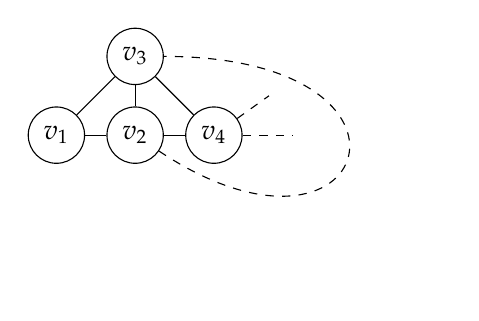
\begin{tikzpicture}
%\tikzstyle{place}=[circle,draw=blue!50,fill=blue!20,thick,inner sep=0pt,minimum size=6mm]
\begin{scope}[every node/.style={circle,draw}]               
    \node (a) at (0,0) {$v_1$};
    \node (b) at (1,0) {$v_2$};
    \node (c) at (1,1) {$v_3$};  
    \node (d) at (2,0) {$v_4$};
        
    \path [-] (a) edge (c);
    \path [-] (a) edge (b);
    \path [-] (b) edge (d);
    \path [-] (c) edge (b);
    \path [-] (c) edge (d);
    %\draw[dashed] (b) -- (2,-0.5);
    \draw[dashed] (d) -- (2.7,0.5);
    \draw[dashed] (d) -- (3,0);        
\end{scope}
\draw[dashed] (b) .. controls (4,-2) and (5,1) .. (c);
\end{tikzpicture}
\caption{A graph $G$ with $\Delta(G)=4$ and $K_3^2\subset G$.}
\label{fg:2k3s}
\end{figure}
\end{lemma}
\begin{proof}
If $\exists u \notin \{v_1,v_4\}$ s.t. $u \in N_G(v_2)\cap N_G(v_3)$, then $H=G[\{v_1,v_2,v_3,v_4,u\}]\subset G$ is triangulated and $E(H)\cap E(G\setminus H)=\emptyset$. Hence, $G'$ is moral. If there exists no such a node $u$, assuming $G'$ is not moral. Without loss of generality, assume $N_G(v_4)=\{v_2,v_3\}$ and $H'=G'[V\setminus \{v_1,v_2,v_3,v_4\}]$ s.t. $D_{H'}(w)\neq \emptyset, \forall w\in V(H')$. Let $G'' = (V(G'), E(G')\setminus\{v_2v_3\})$, then $D_{G''}(v_4)\neq \emptyset$. $N_G(v_4)=\{v_2,v_3\}$ implies $D_{G''}(v_2)\neq \emptyset, D_{G''}(v_3)\neq \emptyset$. Hence, $D_{G''}(w)\neq \emptyset, \forall w\in V(G'')$. Therefore, $G''$ is not moral. Without loss of generality, assuming $\alpha^{-1}(v_1)=1$ so $\nexists \epsilon_{\alpha}(v_1) \subset E(N_G(v_1))$ s.t. $(V \setminus \{v_1\}, E \setminus \epsilon_{\alpha}(v_1))$ is moral. This contradicts with $G$ being moral. \qed
\end{proof}

\begin{figure}[H]
\centering
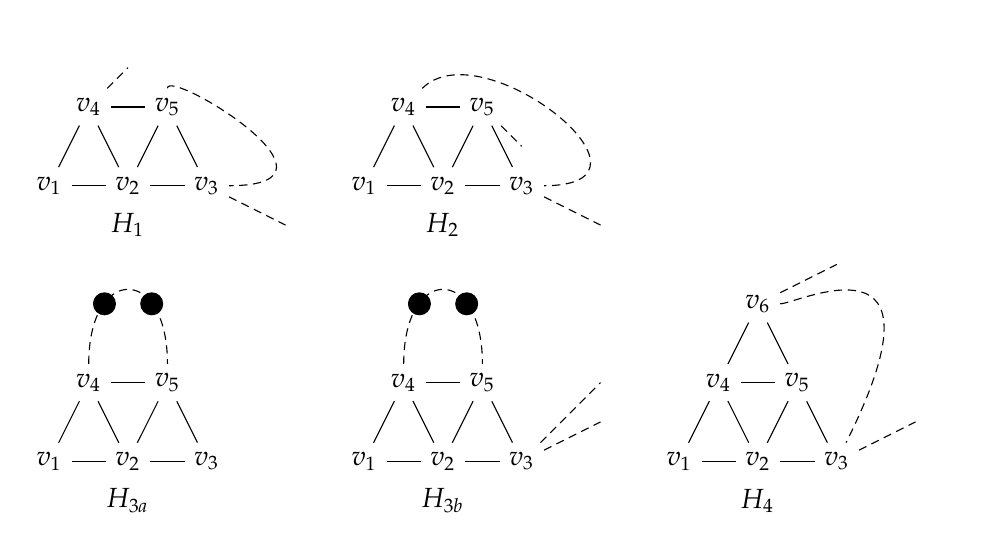
\begin{tikzpicture}
%\tikzstyle{place}=[circle,draw=blue!50,fill=blue!20,thick,inner sep=0pt,minimum size=6mm]
\begin{scope}              
    \node (A) at (-0.5,-2) {$v_1$};
    \node (B) at (1.5,-2) {$v_3$};
    \node (H) at (0,-1) {$v_4$};
    \node (I) at (1,-1) {$v_5$};
    \node (J) at (0.5,-2) {$v_2$};               
    \path [-] (A) edge (J);
    \path [-] (A) edge (H);
    \path [-] (B) edge (I);
    \path [-] (B) edge (J);
    \path [-] (H) edge (I);
    \path [-] (H) edge (J);
    \path [-] (I) edge (J); 
    \path [densely dashed] (H) edge (0.5,-0.5);
    \path [densely dashed] (B) edge (2.5,-2.5);
    
\end{scope}
\draw[densely dashed] (I) .. controls (1,-0.5) and (3.5,-2) .. (B);
\node at (0.5,-2.5) {$H_1$};

\begin{scope}              
    \node (A) at (3.5,-2) {$v_1$};
    \node (B) at (5.5,-2) {$v_3$};
    \node (H) at (4,-1) {$v_4$};
    \node (I) at (5,-1) {$v_5$};
    \node (J) at (4.5,-2) {$v_2$};               
    \path [-] (A) edge (J);
    \path [-] (A) edge (H);
    \path [-] (B) edge (I);
    \path [-] (B) edge (J);
    \path [-] (H) edge (I);
    \path [-] (H) edge (J);
    \path [-] (I) edge (J); 
    \path [densely dashed] (B) edge (6.5,-2.5); 
    \path [densely dashed] (I) edge (5.5,-1.5);       
\end{scope}
\draw[densely dashed] (H) .. controls (5,0) and (7.5,-2) .. (B);
\node at (4.5,-2.5) {$H_2$};

\begin{scope}
    \node (a) at (3.5-4,-5.5) {$v_1$};
    \node (b) at (5.5-4,-5.5) {$v_3$};
    \node (h) at (4-4,-4.5) {$v_4$};
    \node (i) at (5-4,-4.5) {$v_5$};
    \node (j) at (4.5-4,-5.5) {$v_2$};           
    \path [-] (a) edge (j);
    \path [-] (a) edge (h);
    \path [-] (b) edge (i);
    \path [-] (b) edge (j);
    \path [-] (h) edge (i);
    \path [-] (h) edge (j);
    \path [-] (i) edge (j);
    \draw[densely dashed] (h) .. controls (0,-3) and (1,-3) .. (i);
    \foreach \Point in {(0.2,-3.5), (0.8,-3.5)}{
    \node[circle,draw,fill=black,minimum size=0.5mm,inner sep=0.3pt] at \Point {\textbullet};}
\end{scope}


\node at (0.5,-6) {$H_{3a}$};

\begin{scope}
    \node (a) at (3.5,-2-3-0.5) {$v_1$};
    \node (b) at (5.5,-5-0.5) {$v_3$};
    \node (h) at (4,-1-3-0.5) {$v_4$};
    \node (i) at (5,-1-3-0.5) {$v_5$};
    \node (j) at (4.5,-2-3-0.5) {$v_2$};           
    \path [-] (a) edge (j);
    \path [-] (a) edge (h);
    \path [-] (b) edge (i);
    \path [-] (b) edge (j);
    \path [-] (h) edge (i);
    \path [-] (h) edge (j);
    \path [-] (i) edge (j);
    \path [densely dashed] (b) edge (6.5,-4.5-0.5);
    \path [densely dashed] (b) edge (6.5,-4-0.5);  
    \foreach \Point in {(4.2,-3.5), (4.8,-3.5)}{
    \node[circle,draw,fill=black,minimum size=0.5mm,inner sep=0.3pt] at \Point {\textbullet};}  
\end{scope}
\draw[densely dashed] (h) .. controls (4,-2.5-0.5) and (5,-2.5-0.5) .. (i);
\node at (4.5,-5.5-0.5) {$H_{3b}$};

\begin{scope}
	\node (A) at (-0.5+8,-2-3-0.5) {$v_1$};
    \node (B) at (1.5+8,-2-3-0.5) {$v_3$};
    \node (F) at (0.5+8,0-3-0.5) {$v_6$};
    \node (H) at (0+8,-1-3-0.5) {$v_4$};
    \node (I) at (1+8,-1-3-0.5) {$v_5$};
    \node (J) at (0.5+8,-2-3-0.5) {$v_2$};  
	\path [-] (A) edge (J);
    \path [-] (A) edge (H);
    \path [-] (B) edge (I);
    \path [-] (B) edge (J);
    \path [-] (F) edge (H);
    \path [-] (F) edge (I);
    \path [-] (H) edge (I);
    \path [-] (H) edge (J);
    \path [-] (I) edge (J);
    \path [densely dashed] (F) edge (9.5,-2.5-0.5);
    \path [densely dashed] (B) edge (10.5,-4.5-0.5);    
\end{scope}
\draw[densely dashed] (F) .. controls (9,-3-0.5) and (11,-2-0.5) .. (B);
\node at (8.5,-5.5-0.5) {$H_4$};
\end{tikzpicture}
\caption{A list of all possible induced subgraphs $H \subset G$ with $\Delta(G)=4$, where $K_3^3\subset H$. Each dotted edge connects a node to a subgraph (possibly empty) of $G$. $H_4$ is a special case of $H_3$ when $N_{G}(v_4)\cap N_{G}(v_5)=\{v_2,v_6\}$. Without loss of generality, assume $D_G(v_1)=\emptyset$.}
\label{fg:3k3s}
\end{figure}

\begin{lemma}
\label{lm:3k3s_a}
Let $G=(V,E)$ be a moral graph with $\Delta(G)=4$ and $K_3^3\subset G$ as shown in Figure \ref{fg:3k3s}. If $\max\{|P|\mid P=v_4\dots v_5 \in G[V-\{v_1,v_2,v_3\}]\} \le 2$ and $D_G(v_1)=\emptyset$, then $G'=(V-\{v_1\}, E-E(G[N[v_1]]))$ is moral.  
\end{lemma}
\begin{proof}
The lemma assumes $G$ contains a subgraph that is identical to either $H_1$, $H_2$ or $H_4$. It is then safe to remove $v_1$ and $v_2v_4$, because $v_4v_5 \notin C_m \subset G[V\setminus \{v_1,v_2,v_3\}]$ for $m \ge 4$. Hence, $K_3\subset G'$ is moral by Lemma \ref{lm:1k3}. \qed
\end{proof}

\begin{algorithm}[]
\caption{Checking morality for maximum degree $4$ graphs}
\label{alg:d_wrs_deg4}
\begin{algorithmic}[]
	\Require{a graph $G=(V,E)$ with $\Delta(G)=4$}
    
    \If{$\exists x$ s.t. $D_G(x)=\emptyset,d_G(x)=4$}
       \State \Return{TRUE}
    \EndIf
    
    \While {$D(G)=\emptyset$}
    
    \If{$\exists x$ s.t. $D_G(x)=\emptyset, d_G(x)=1$}
       \State $G=G[V-\{x\}]$
    \ElsIf{$\exists x$ s.t. $D_G(x)=\emptyset,d_G(x)=3$}
       \State $G=(V-\{x\},E-E(G[N_G[x]]))$
    \ElsIf{$\exists x \in K_3^m$ s.t. $D_G(x)=\emptyset$ for $m \ge 4$} \Comment{reduce long stack}
       \State $G=(V-\{x\},E-E(G[N_G[x]]))$
    \ElsIf{$\exists x \in K_3$ s.t. $D_G(x)=\emptyset$}
       \State $G=(V-\{x\},E-E(G[N_G[x]]))$
    \ElsIf{$\exists x \in K_3^2$ s.t. $D_G(x)=\emptyset$}
       \State $G=G[V-\{x\}]$
    \Else \Comment{all simplicial $x \in K_3^3$}
    	\If{$\max\{|P|\mid P=v_4\dots v_5 \in G[V-\{v_1,v_2,v_3\}]\} \le 2$}
    		\State $G=(V-\{x\},E-E(G[N_G[x]]))$
    	\Else 
    		\If{$\exists y \in K_3^3$ s.t. $D_G(y)=\emptyset$ and $|N_G(x)\cap N_G(y)|=1$} \Comment{$H_{3a}\in G$}
       			\State $G=G[V-\{x,y\}]$
   			\Else \Comment{$H_{3b} \in G$}
       			\State $G=(V-\{x\},E-E(G[N_G[x]]))$
       		\EndIf
    	\EndIf
    	
       
    \EndIf
    
    \EndWhile
    
    \State \Return{FALSE}
    
\end{algorithmic}
\end{algorithm}

\begin{theorem}
\label{thm:deg4}
The morality of maximum degree $4$ graphs can be checked by Algorithm \ref{alg:d_wrs_deg4}.
\end{theorem}
\begin{proof}
A part of the algorithm has been proven correct by Lemma \ref{lm:deg1_4_3}, Lemma \ref{lm:1k3}, Lemma \ref{lm:2k3s} and Lemma \ref{lm:3k3s_a}. If $K_3^m \subset G$ for $m \ge 4$, removing $x$ and $E(G[N_G[x]])$ reduces $m$ by 2 at a time. It remains to show that the two operations for the cases of $x \in H_{3a}$ and $x \in H_{3b}$ are correct. 

Assume $G$ is moral but $G'$ is not. If $x\in H_{3a}$, without loss of generality, assume $H \in \{H_1=G[V\setminus \{v_1,v_2,v_3\}], H_2=G[V\setminus \{v_1,v_2,v_3,v_4,v_5\}]\}$ s.t. $D_H(w) \neq \emptyset, \forall w \in V(H)$. It is easy to see that for any $\emptyset \neq S \subset \{v_2v_4,v_2v_5\}$, the subgraph $G''=(V \setminus \{v_1,v_3\},E(G[V \setminus \{v_1,v_3\}])-S)$ satisfies $H_1 \subset G''$ and $E(G''\setminus H_1) \cap E(H_1) = \emptyset$. Hence, $G''$ is not moral. If $x \in H_{3b}$, $D_{G'}(v_2)=\emptyset$. Without loss of generality, assume $H =(V(G')\setminus \{v_2\},E(G[V(G')\setminus \{v_2\}])\setminus S)$ where $S \subset \{v_3v_5\}$ s.t. $D_H(w) \neq \emptyset, \forall w \in V(H)$. Let $G''=(V\setminus \{v_1\}, E(G[V\setminus \{v_1\}]))$, then $D_{G''}(v_2)\neq \emptyset$, so $G''$ is not moral. Hence, if $G$ and $G'$ both are moral.

The complexity of Algorithm \ref{alg:d_wrs_deg4} ...

\end{proof}

\section{Conclusion}
In this paper, we have drawn an one-to-one correspondance between Markov blankets consistency and graph morality. We have presented polynomial time algorithms for checking graph morality for graphs with maximum degree $3$ and $4$. We have also built a polynomial time reduction based upon \cite{verma1993deciding} from the 3-CNF problem to graph morality for graphs with maximum degree $5$ and above, and consequently proved that the problem is NP-complete. Furthermore, we introduced two new concepts-weak recursively simplicial graphs and perfect elimination kit-to help proving the complexity of checking morality and for future research on related toipics. 


\newpage
%Since the atomic cycles in a graph can be enumerated in at most $O(m^2)$ time (citation!!!), both remarks can be run efficiently to spot non-moral graphs. 
\section{Polytree}
\begin{proposition}
\label{prop:moral_of_pt_chordal}
Let $T=(V,E)$ be a polytree and $F$ be the moral graph of $T$. Then $F$ is a chordal graph. 
\end{proposition}
\begin{proof}
Assuming $F$ is not a chordal graph, there must exist a chordless $C_m \subset F$ for $m\ge 4$. $F$ being moral implies that the $C_m$ shares an edge with a simplicial clique $K_n$ for $n \ge 3$. Hence, there are multiple paths between a node in the $C_m$ and the simplicial node in the $K_n$ via different neighbours of the simplicial node. Henc, the assumption leads to a contradiction to $T$ being singly connected. \qed
\end{proof}

The converse of Proposition \ref{prop:moral_of_pt_chordal} is not true. For example, the chordal moral graph in Figure \ref{fg:chordal_over_4nodes} comes from a non-singly connected DAG. 
\begin{figure}[H]
\centering
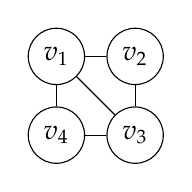
\begin{tikzpicture}
%\tikzstyle{place}=[circle,draw=blue!50,fill=blue!20,thick,inner sep=0pt,minimum size=6mm]
\begin{scope}[every node/.style={circle,draw}]           
    \node (A) at (2,2) {$v_1$};
    \node (B) at (3,2) {$v_2$};
    \node (C) at (3,1) {$v_3$};
    \node (D) at (2,1) {$v_4$};
    
    \path [-] (A) edge (B);
    \path [-] (A) edge (D);
    \path [-] (C) edge (D);
    \path [-] (C) edge (B);
    \path [-] (A) edge (C);
\end{scope}
\end{tikzpicture}
\caption{A chordal graph that comes from moralizing a non-singly connected DAG.}
\label{fg:chordal_over_4nodes}
\end{figure}

\begin{corollary}
Let $B_X$ be a set of Markov blankets over a variable set $X$. The problem of testing if $B_X$ is consistent with a polytree tree is in polynomial time.
\end{corollary}
\begin{proof}
Chordality can be verified in polynomial time \cite{tarjan1984simple}. \qed
\end{proof}

\textbf{Idea:} Since it is in polynomial time to check if a set of learned $B_X$ is consistent with a DAG or not, we could start the structure discovery process by learning a polytree over all variables in $X$. Then gradually build up a DAG from a polytree. In addition, because a polytree is a subset of DAGs, so there would be less number of consistent polytrees to a chordal graph than consistent DAGs to a WRS graph. 


\newpage
\section{Minimal moralization}
From now on, we try to develop polynomial time algorithms for finding the maximal moral subgraph or the minimal moral supergraph of a given non-moral graph $F$.

\begin{definition}
A \textbf{simple cycle} $C$ in a graph is a closed walk such that each node in $V(C)$ is only visited once except for the starting node.
\end{definition}

\begin{definition}
An \textbf{induced simple cycle} in a graph $F$ is a simple cycle that is an induced subgraph of $F$. 
\end{definition}

\begin{remark}
The number of induced simple cycles of length 4 or more in $F$ gives an upper bound of the number of edges to be added/removed from $F$.
\end{remark}

\begin{remark}
The minimal moral supergraph problem is NP-complete, because if it is polynomial then we can run an algorithm to find the minimal moral supergraph of a graph $F$ and comparing it with $F$. This will identify if $F$ is moral or not in polynomial time. 
\end{remark}

Both minimum triangulation and maximum chordal subgraph seem to be only solvable in NP-complete time complexity. But minimal triangulation and maximal subgraphs seem to be solvable in efficient time. 

Minimal triangulation is related to minimal separator. A vertext $S\subset V$ is a \textbf{separator} if $F[V\setminus S]$ is disconnected. Given two vertices $u,v\in V$, $S$ is a $u,v$-separator if $u$ and $v$ belong to different connected components of $F[V\setminus S]$. $S$ is called a minimal $u,v$-separator if $S$ has no proper subset that separates $u$ and $v$. A vertex $S\subset V$ is a \textbf{minimal separator} of $F=(V,E)$ if $\exists u, v \in V$ s.t. $S$ is a minimal $u,v$-separator. 
 

\begin{itemize}
\item Chordality is not preserved under graph complementation, so finding the maximal chordal subgraph is not reducible to finding minimal chordal supergraphs. This is the same for morality, I've just randomly generated some graphs and their complements, they nont always have the same morality. 
\item Chordality is a hereditary property. That is, if a graph $F=(V,E)$ is chordal, the subgraph of $F$ induced by $V\setminus \{x\}$ is also chordal where $x$ is a simplicial node in $F$. But morality is not a hereditary property, because the induced subgraph after removing a simplicial node from $F$ may or may not be moral. 
\item Since checking morality in general is NP-complete, I suspect that the finding the minimal triangulation of a graph is al NP-complete. For otherwise, we could find the minimal triangulation of a graph and compare it with the original graph. If they are identical, then the original graph is NP-complete. 
\item Run backtracking algorithm on a graph, if the algorithm stucks, add pick a node with the minimum degree and add its deficiency. This way will result a graph that is moral (and perhaps chordal), but won't be a minimal moral supergraph. A moral graph is a minimal supergraph of a graph $F$ if there is no another moral graph that is a proper subgraph of it. 
\item Different ordering will result in different moral supergraph, hence the choice of a node to eliminate at each step is crucial. 
\end{itemize}

\subsection{Preliminary}
In this section, we define some new concepts of moral graphs which will be used later to help finding minimal moralization of an undirected graph. Most of these concepts are introduced in parallel with similar concepts for chordal graphs, but generalized to moral graphs. 

\begin{definition}
A graph $H=(V,E\cup F)$ is called a \textbf{moralization} of an undirected graph $G=(V,E)$ if $H$ is moral. 
\end{definition}

Without loss of generality, assuming $F\neq \emptyset$ and $E\cap F=\emptyset$. Every edge $e\in E\cup F$ is either an edge of the underlying graph $G$ or a \textit{fill edge} in $F$. 

\begin{definition}
Let $G=(V,E)$ be a graph, and $H=(V,E\cup F)$ be a moral graph with $F\neq \emptyset$ and $E\cap F=\emptyset$. $H$ is a \textbf{minimal moralization} of $G$ if $(V,E\cup F')$ is non-moral $\forall F' \subsetneq F$. It is the \textbf{minimum moralization} if $\nexists E'$ with $|E'| < |F|$ s.t. the graph $(V,E\cup E')$ is moral. 
\end{definition}
Sometimes people also refer the set of fill edges $F$ as a minimal moralization instead of the graph $H$. The following is an  example of a minimal and minimum moralizations. 
\begin{figure}[H]
\centering
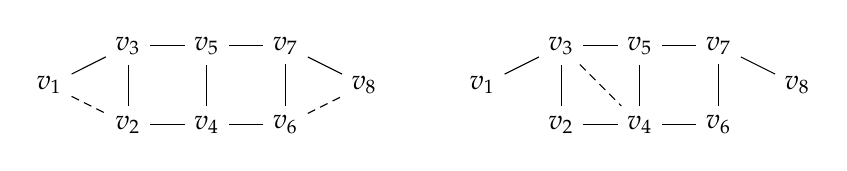
\begin{tikzpicture}
%\tikzstyle{place}=[circle,draw=blue!50,fill=blue!20,thick,inner sep=0pt,minimum size=6mm]
\begin{scope}         
    \node (a) at (-1,0.5) {$v_1$};
    \node (b) at (0,0) {$v_2$};   
    \node (c) at (0,1) {$v_3$};
    \node (d) at (1,0) {$v_4$};
    \node (e) at (1,1) {$v_5$};
    \node (f) at (2,0) {$v_6$};
    \node (g) at (2,1) {$v_7$};
    \node (h) at (3,0.5) {$v_8$};
            
    \path [-] (a) edge (c);
    \path [densely dashed] (a) edge (b);
    \path [-] (b) edge (c);
    \path [-] (b) edge (d);
    \path [-] (c) edge (e);
    \path [-] (d) edge (e);
    \path [-] (d) edge (f);
    \path [-] (e) edge (g);
    \path [-] (f) edge (g);
    \path [-] (g) edge (h);
    \path [densely dashed] (f) edge (h);
\end{scope}
\begin{scope}         
    \node (a) at (-1+5.5,0.5) {$v_1$};
    \node (b) at (0+5.5,0) {$v_2$};   
    \node (c) at (0+5.5,1) {$v_3$};
    \node (d) at (1+5.5,0) {$v_4$};
    \node (e) at (1+5.5,1) {$v_5$};
    \node (f) at (2+5.5,0) {$v_6$};
    \node (g) at (2+5.5,1) {$v_7$};
    \node (h) at (3+5.5,0.5) {$v_8$};
            
    \path [-] (a) edge (c);
    \path [densely dashed] (c) edge (d);
    \path [-] (b) edge (c);
    \path [-] (b) edge (d);
    \path [-] (c) edge (e);
    \path [-] (d) edge (e);
    \path [-] (d) edge (f);
    \path [-] (e) edge (g);
    \path [-] (f) edge (g);
    \path [-] (g) edge (h);
\end{scope}
\end{tikzpicture}
\caption{An example of a minimal (left) and minimum (right) moralizations.}
\label{fg:mini_moral}
\end{figure}

\begin{definition}
An \textbf{ordering} of a graph $G=(V,E)$ with $n$ vertices is a bijection $\alpha: \{1, \dots, n\} \leftrightarrow V$. 
\end{definition}
We use $\alpha$ to denote the ordering of $G$. $\alpha^{-1}(v)$ is the number assigned to the node $v$ according to $\alpha$. An \textit{elimination ordering} is an ordering that gives as an input to the Elimination Game (EA) algorithm \cite{fulkerson1965incidence} to obtain a triangulated graph $G_{\alpha}^+$.  

\begin{definition}
An \textbf{excess} of a graph $G=(V,E)$ is a bijection $\epsilon_{\alpha}: \alpha \leftrightarrow \{\epsilon_{\alpha}(v_1), \dots, \epsilon_{\alpha}(v_n)\}$ where $\epsilon_{\alpha}(v_i) \subset E(G[N(v_i)])$.
\end{definition}
We use $\epsilon_{\alpha}$ to denote the excess of $G$ and $\epsilon_{\alpha}(v_i)$ to denote the excess of $v_i$ according to the ordering $\alpha$. The composition of an ordering and an excess forms an \textit{elimination kit} denoted by $\kappa=(\alpha,\epsilon_{\alpha})$ that can be used to extend the EA algorithm to graph moralization. 

\iffalse
\begin{definition}
Let $\kappa=(\alpha,\epsilon_{\alpha})$ be an elimination kit of a graph $G$. $\kappa$ is \textbf{minimal} if $G_{\kappa}^+$ is a minimal moralization of $G$. 
\end{definition}
\fi

\begin{definition}
Let $\kappa=(\alpha,\epsilon_{\alpha})$ be an elimination kit of a graph $G$. $\kappa$ is \textbf{minimal} if there is no other elimination kit $\kappa'$ s.t. $G_{\kappa'}^+$ is a proper subgraph of $G_{\kappa}^+$. It is \textbf{perfect} if $G_{\kappa}^+=G$. 
\end{definition}

\begin{definition}
Let $G=(V,E)$ be a connected graph. A vertex set $S\subset V$ is a \textbf{separator} if $G[V-S]$ is disconnected. 
\end{definition}

\begin{definition}
A graph $G$ is called \textbf{connected} if there is a path between every pair of vertices in $G$. 
\end{definition}

\begin{definition}
Let $G$ be a graph. A maximal connected subgraph of $G$ is called a \textbf{component} of $G$. 
\end{definition}

\begin{definition}
Given two non-adjacent vertices $u,v$ in a graph $G=(V,E)$. A vertext set $S \subset V$ is a \textbf{$u,v$-separator} if $u$ and $v$ belong to different components of $G[V-S]$. In particular, $S$ is a \textbf{minimal} $u,v$-separator if there exists no proper subset of $S$ that separates $u$ and $v$. 
\end{definition}

\subsection{Characterizations of minimal moralization}
Firstly, we prove that for each minimal moralization $H$ of $G$, there exists a mek $\kappa$ s.t. $H=G_{\kappa}^+$. The consequence of this result is that finding a minimal moralization or a mek are equivalent problems. The result is proved by the same logic as in \cite{ohtsuki1976minimal} for chordal graphs. 
\begin{lemma}
\label{lm:ohtsuki_lm1}
Let $G=(V,E)$ be a graph and $H=(V,E\cup F)$ be a minimal moralization of $G$. Then there exists a minimal elimination kit $\kappa$ s.t. $G_{\kappa}^+=H$. 
\end{lemma}
\begin{proof}
$H$ is moral implies it has a pek $\kappa$. $G \subset H$ implies $G_{\kappa}^+=(V,E\cup F') \subset H$. Since $H$ is minimal, $F'=F$ and consequently $G_{\kappa}^+=H$. Assuming $H$ has another pek $\kappa'$ with $G_{\kappa'}^+ =(V,E\cup E') \subsetneq G_{\kappa}^+$. It entails that $E' \subsetneq F$, which contradicts $H$ being minimal. \qed
\end{proof}

\begin{lemma}
\label{lm:ohtsuki_lm2}
Let $\kappa$ be a minimal elimination kit of a graph $G=(V,E)$. Then $G_{\kappa}^+$ is a minimal moralization of $G$. 
\end{lemma}
\begin{proof}
Assuming $G_{\kappa}^+=(V,E\cup E')$ is not minimal. That is, there exists another set of fill edges $F\subsetneq E'$ with $H=(V,E\cup F)$ being moral. Without loss of generality, assuming $H$ is a minimal. Lemma \ref{lm:ohtsuki_lm1} implies that $\exists \kappa'$ s.t. $G_{\kappa'}^+=H \subsetneq G_{\kappa}^+$. It contradicts with $\kappa$ being a mek. \qed
\end{proof}

\begin{theorem}
\label{thm:ohtsuki_thm1}
A graph $H$ is a minimal moralization of $G$ if and only if there exists a minimal elimination kit $\kappa$ s.t. $H=G_{\kappa}^+$.
\end{theorem}
\begin{proof}
The theorem follow from Lemma \ref{lm:ohtsuki_lm1} and Lemma \ref{lm:ohtsuki_lm2}. \qed 
\end{proof}

\begin{theorem}
A graph is moral if and only if it has a perfect elimination kit. 
\end{theorem}
\begin{proof}
The proof is trivial. \qed
\end{proof}

If there exists a perfect elimination kit (pek) $\kappa$ with $\epsilon_{\alpha} =\emptyset$, then $G$ is chordal and the outputs $G_{\kappa}^+=G_{\alpha}^+$. 

The EA algorithm outputs a moralized graph that possibly contains more edges than needed for moralization. To pursue a smaller moralized graph, the \textit{minimal moralization sandwich problem} looks for a minimal moralization $H$ of $G$ s.t. $G \subseteq H \subseteq G_{\kappa}^+$ for a given elimination kit. 

The following lemmas and theorems are stated and proved in similar ways as those for triangulated graphs in \cite{rose1976algorithmic}. 

\begin{lemma}
\label{lm:rose_lm1}
Let $G=(V,E)$ be a moral graph with a pek $\kappa=(\alpha,\epsilon_{\alpha})$. For any node $x \in V$, the graph $G'=(V,E\cup D_G(x))$ has a pek $\kappa'=(\alpha, \epsilon'_{\alpha})$. 
\end{lemma}  
\begin{proof}
We want to show that for any two distinct edges $\{v_iv_j, v_iv_k\} \subset E\cup D_G(x)-E'$ with $\alpha^{-1}(v_i) < \min \{\alpha^{-1}(v_j), \alpha^{-1}(v_k)\}$, the edge $v_jv_k \in E\cup D_G(x)-E'$ where $E' = \{\epsilon'_{\alpha}(v_1),\dots,\epsilon'_{\alpha}(v_{i-1})\}$ is the set of removed edges up to $v_i$ according to $\kappa'$.

\textit{Case 1:} If $\{v_iv_j, v_iv_k\} \subset E-E'$, since $v_i$ comes before $v_j$ and $v_k$ in $\alpha$, the edge $v_jv_k\in E-E'$ because $\kappa'$ is perfect.

\textit{Case 2:} If $\{v_iv_j, v_iv_k\} \subset D_G(x)-E'$, then $\{v_i,v_j,v_k\} \subset N_G(x)$ so $v_jv_k \in D_G(x)$. It remains to show that $v_jv_k \notin E'$. If there is a node $v_l$ with $\alpha^{-1}(v_l) < \alpha^{-1}(v_i)$ and $v_jv_k\in \epsilon_{\alpha}(v_l)$ because it is in a cycle, then it is possible for $v_jv_k \in \epsilon'_{\alpha}(v_i)$ to break the same cycle. 
\begin{figure}[H]
\centering
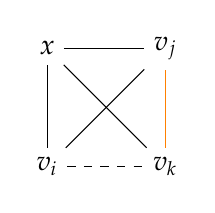
\begin{tikzpicture}
%\tikzstyle{place}=[circle,draw=blue!50,fill=blue!20,thick,inner sep=0pt,minimum size=6mm]
\begin{scope}         
    \node (a) at (0,0) {$v_i$};
    \node (b) at (0,1.5) {$x$};   
    \node (c) at (1.5,0) {$v_k$};
    \node (d) at (1.5,1.5) {$v_j$};
            
    \path [-] (a) edge (b);
    \path [dashed] (a) edge (c);
    \path [-] (a) edge (d);
    \path [-] (b) edge (c);
    \path [-] (b) edge (d);
    \path [-][orange] (c) edge (d);
\end{scope}
\end{tikzpicture}
\caption{An example of case 3. The solid lines are in $E$. The dashed is in $D(x)$. The orange is the edge we want to prove to belong to $E\cup D(x)$.}
\label{fg:case3}
\end{figure}
\textit{Case 3:} If $v_iv_j \in E-E'$ and $v_iv_k \in D_G(x)-E'$, then $\{v_i,v_k\}\subset N_G(x)$. If $x=v_j$ then $v_jv_k \in E$. Otherwise (Figure \ref{fg:case3}), we have $\alpha^{-1}(v_i) < \alpha^{-1}(x)$ because $v_iv_k \in D_G(x)$. If so, $xv_j \in E$ because $\{x, v_j\} \subset N_G(v_i)$. It then follows that $v_jv_k \in E\cup D_G(x)$ because $\{v_j,v_k\} \subset N_G(x)$. For the same argument in case 2, $v_jv_k \notin E'$. \qed
\end{proof}

\begin{corollary} 
\label{cor:rose_cor2}
Let $G=(V,E)$ be a moral graph and $x$ be any node with $D_G(x)=\emptyset$. Then there is a pek $\kappa=(\alpha,\epsilon_{\alpha})$ of $G$ with $\alpha(1) = x$.
\end{corollary}
\begin{proof}
Let $R=\{x \mid D_G(x)=\emptyset\}$. Morality implies that $|R|\ge 1$. If $|R|=1$, it is certain that $\alpha(1)=x$. Otherwise, for any $x\in R$, there is a different pek $\kappa=(\alpha,\epsilon_{\alpha})$ for $G$ with $\alpha(1)=x$.  \textcolor{red}{Not quite a proof!} \qed
\end{proof}

\begin{corollary}
\label{cor:rose_cor1}
Let $G=(V,E)$ be a moral graph with a pek $(\alpha, \epsilon_{\alpha})$ and $x$ is any node in $G$. Then there exists a pek $\kappa'=(\alpha,\epsilon'_{\alpha})$ for the graph $G'=(V,E\cup D_G(x))$ s.t. the subgraph $G'_x = (V-\{x\},E(G[V\setminus \{x\}])\cup D_G(x)-\epsilon'_{\alpha}(x))$ is also moral. 
\end{corollary}
\begin{proof}
Lemma \ref{lm:rose_lm1} implies that $G'=(V,E\cup D_G(x))$ is moral. Corollary \ref{cor:rose_cor2} suggests that $G'$ has a pek $\kappa'=(\alpha,\epsilon'_{\alpha})$ with $\alpha(1)=x$. Hence, $G'_x = (V-\{x\},E(G[V\setminus \{x\}])\cup D_G(x)-\epsilon'_{\alpha}(x))$ is also moral because of the hereditary property of morality. \qed
\end{proof}

\begin{lemma}
\label{lm:rose_lm2}
Let $G=(V,E)$ and $H=(V,E\cup F)$ be moral graphs with peks $(\alpha,\epsilon_{\alpha})$ and $(\beta,\epsilon_{\beta})$ respectively and $F\neq \emptyset$, $E \cap F=\emptyset$. Then there exists at least one edge $f=uv \in F$ with $\beta^{-1}(u) < \beta^{-1}(v)$ s.t. $H-f-E'=(V,E\cup F-\{f\}-E')$ is moral, where $E'=\{vw \in F \mid vw \in \epsilon_{\beta}(u)\}$.
\end{lemma}
\begin{proof}
We prove the lemma by induction on the number of nodes. When $|V| \le 3$, all graphs are moral so the lemma is true. Assuming it is true for $|V|=n-1 \ge 4$, we want to show that the lemma is also true for $n$ nodes. Let $R=\{x\mid D_G(x)=\emptyset\}$ and $S=\{x\mid D_{H}(x)=\emptyset\}$. Since both graphs are moral, none of these sets is empty. The proof is divided into two cases, depending on whether or not there exists a node $u \in S$ with $f=uv \in F$.

\textit{Case 1:} $\exists u \in S$ with  $f=uv\in F$. Since $u\in S$, Corollary \ref{cor:rose_cor2} suggests $H$ has a pek $(\beta,\epsilon_{\beta})$ with $\beta(1)=u$. Furthermore, $N_H(u)-\{v\}$ still forms a clique after removing $f$ and $E'$ that contains the edges between $v$ and the other neighbours of $u$. Therefore, $H-f-E'$ is moral with a pek $(\beta,\epsilon_{\beta}-E')$. 

\textit{Case 2:} $\nexists u \in S$ with  $f=uv\in F$. In this case, we want to show that $\exists x\in S$ with $F\nsubseteq D_G(x)$. (\textcolor{red}{an exmaple is sufficient}?) Assuming $\nexists x \in S$. That is, $\forall x\in S$ satisfy $F\subseteq D_G(x)$. Being in $S$ implies $D_G(x) \subseteq F$, so $F=D_G(x)$. For any node $x\in R$, Corollary \ref{cor:rose_cor2} suggests there is a pek $(\alpha, \epsilon_{\alpha})$ for $G$ with $\alpha(1)=x$. Lemma \ref{lm:rose_lm1} implies $(\alpha,\epsilon'_{\alpha})$ is a pek for $(V,E\cup D(x))=(V,E\cup F)=H$, hence $x\in S$. Therefore, for any node in $R$, it is also in $S$. But $x\in R$ implies $D_G(x)=\emptyset$. In conjunction with $F\neq \emptyset$, it entails that $F \nsubseteq D_G(x)$ that is a contradiction. Therefore, if case 2 is true $\exists x\in S$ with $F\nsubseteq D_G(x)$ (Figre \ref{fg:case2}). 
\begin{figure}[H]
\centering
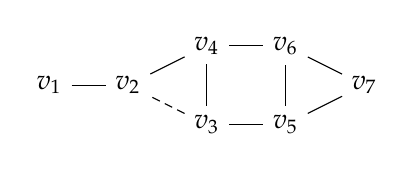
\begin{tikzpicture}
%\tikzstyle{place}=[circle,draw=blue!50,fill=blue!20,thick,inner sep=0pt,minimum size=6mm]
\begin{scope}          
    \node (a) at (-1,0.5) {$v_1$};
    \node (b) at (0,0.5) {$v_2$};   
    \node (c) at (1,0) {$v_3$};
    \node (d) at (1,1) {$v_4$};
    \node (e) at (2,0) {$v_5$};
    \node (f) at (2,1) {$v_6$};    
   	\node (g) at (3,0.5) {$v_7$};
            
    \path [-] (a) edge (b);
    \path [densely dashed] (c) edge (b);
    \path [-] (c) edge (d);
    \path [-] (d) edge (b);
    \path [-] (c) edge (e);
    \path [-] (d) edge (f);
    \path [-] (e) edge (f);
    \path [-] (e) edge (g);
    \path [-] (f) edge (g);
\end{scope}
\end{tikzpicture}
\caption{An example of case 2, where $F=\{v_2v_3\}$, $R=S=\{v_1,v_7\}$. Each node $x\in S$ satisfies that $F\nsubseteq D_G(x)$.}
\label{fg:case2}
\end{figure}
For such a node $x \in S$, Lemma \ref{lm:rose_lm1} and Corollary \ref{cor:rose_cor1} imply the following moral graphs and peks
\begin{align*}
G &= (V,E) \text{ with } (\alpha,\epsilon_{\alpha}) \\
G' &=(V,E\cup D_G(x)) \text{ with } (\alpha, \epsilon'_{\alpha}) \\
G'_x&=(V-\{x\}, E(G[V-\{x\}])\cup D_G(x)-\epsilon'_{\alpha}(x))\\
H &= (V,E\cup F) \text{ with } (\beta, \epsilon_{\beta}) \\
H' &=(V,E\cup F \cup D_G(x)) \text{ with } (\beta, \epsilon'_{\beta})\\
H'_x&=(V-\{x\}, E(G[V-\{x\}])\cup F\cup D_G(x)-\epsilon'_{\beta}(x)).
\end{align*}
$F\nsubseteq D(x)$ entails $G' \subsetneq H'$. Since $\alpha(1)=\beta(1)=x$, there exist excesses s.t. $\epsilon'_{\beta}(x) \subseteq \epsilon'_{\alpha}(x)$. Let $F'=E(H'_x)-E(G'_x)=(F-D(x))\cup (\epsilon'_{\alpha}(x)-\epsilon'_{\beta}(x))$. It follows that $F'\neq \emptyset$ and $F' \cap E(G'_x)=\emptyset$. By the inductive hypothesis, there exists an edge $f=uv \in F'$ with $\beta^{-1}(u)<\beta^{-1}(v)$ s.t. $H'_x-f-E'$ is moral where $E'=\{vw \in F' \mid vw \in \epsilon'_{\beta}(u)\}$. Neither of $\{f\}$ or $E'$ is in $D(x)$, so adding $\{x\}$ and $\epsilon'_{\beta}(x)$ back to $H'_x$ does not change the morality of $H'-f-E'$. \qed
\end{proof}

The following theorem is one of the main results for this section. 
\begin{theorem}
Let $G=(V,E)$ be a graph, and $G'=(V,E\cup F)$ be a moralization of $G$ with $E\cap F=\emptyset$. Then $F$ is a minimal moralization if and only if there exists a pek $(\beta,\epsilon_{\beta})$ s.t. for each $f=uv \in F$ with $\beta^{-1}(u) < \beta^{-1}(v)$, $G'-f-E'=(V,E\cup F -\{f\}-E')$ is not moral, where $E'=\{vw \in F \mid vw \in \epsilon_{\beta}(u)\}$.
\end{theorem}
\begin{proof}
The theorem is proved by the definition of minimal moralization and Lemma \ref{lm:rose_lm2}. \qed 
\end{proof}
A consequence of the theorem is that if both $F$ and $H$ are moralizations of $G$ and $F \subsetneq H$, then there is a sequence of subsets of edges $\{f\}\cup E'$ that can be removed from $H$ one by one, such that the resulting graph after each removal is moral. 

Every minimal separater of a chordal graph is a clique \cite{dirac1961rigid}. This result, however, is not true for moral graphs which are more general than chordal graphs. The following theorem states the relation between minimal separater and moral graphs. 
\begin{theorem}
A graph $G=(V,E)$ is moral if and only if there exists an elimination kit $\kappa=(\alpha,\epsilon_{\alpha})$ s.t. for every pair of non-adjacent vertices $u,v\in V$ with $i=\min\{\alpha^{-1}(u),\alpha^{-1}(v)\}$, the minimal $u,v$-separator is a clique in $G^i=G-\{\alpha(1),\dots,\alpha(i-1)\}-\{\epsilon_{\alpha}(\alpha(1)),\dots,\epsilon_{\alpha}(\alpha(i-1))\}$.
\end{theorem}
\begin{proof}
If $G$ is moral with $n$ nodes, there exists a pek $\kappa=(\alpha, \epsilon_{\alpha})$. Without loss of generality, assuming $i=\alpha^{-1}(u) < \alpha^{-1}(v)$ for any two nodes $u,v \in V$. In addition, $uv \notin E$ implies that $v$ is separated from $u$ by $S\subseteq N_G(u)$. Since $\kappa$ is a pek, $u$ must be a simplicial node in the subgraph $G^i$. Therefore, $N_G(u)$ forms a clique and consequently any subset of it is also a clique. 

To prove the sufficient condition, assume $G$ is not moral. That is, $\exists H \subset G$ a mpe subgraph s.t. $D(H)\neq \emptyset$. Hence, $\exists C_m \subset H$ an atomic cycle for $m \ge 4$ st. $\exists u,v \in V(C_m)$ with $uv \notin E(C_m)$. Therefore, the minimal $u,v$-separator is not a clique, which is a contradiction. \qed
\end{proof}


\subsection{Minimal moralization algorithms}
We have defined $G^i=G-\{\alpha(1),\dots,\alpha(i-1)\}-\{\epsilon_{\alpha}(\alpha(1)),\dots,\epsilon_{\alpha}(\alpha(i-1))\}$, which can be interpreted as the resulting graph in step $i$ of the EG algorithm. 
\begin{definition}
Let $G=(V,E)$ be a graph and $\kappa=(\alpha,\epsilon_{\alpha})$ be an eliminiation kit of $G$. If $D_{G^i}(\alpha(i))=\emptyset$ for $i \in [1,p]$ and $\nexists \kappa'=(\beta,\epsilon_{\beta})$ s.t. $D_{G^i}(\beta(i))=\emptyset$ for $i \in [1,q]$ and $\{\alpha(1),\dots,\alpha(p)\}\subsetneq \{\beta(1),\dots,\beta(q)\}$ where $p,q \le |V|$, then $\kappa$ is called a \textbf{maximal perfect elimination kit} of $G$.
\end{definition}
If $\kappa$ is a maximal perfect elimination kit of $G$ with $D_{G^i}(\alpha(i))=\emptyset$ for $i \in [1,p]$, then $H=G-\{\alpha(1),\dots,\alpha(p)\}-\{\epsilon_{\alpha}(\alpha(1)),\dots,\epsilon_{\alpha}(\alpha(p))\}$ is called a \textit{minimal perfect eliminated (mpe) subgraph} of $G$. If $\kappa$ is a pek, then the mpe subgraph of $G$ is empty. If $D(G)\neq \emptyset$, then $G$ is the mpe subgraph of itself. 

\textbf{Conjecture:} If $H\subset G$ is a mpe subgraph of $G$, then a minimal moralization of $H$ is also a minimal moralization of $G$. If $G$ has many mpe subgraphs and none of them is overlapped, then this seems trivial. But if $\exists H_1,H_2\subset G$ are both mpe of $G$ and $H_1\cap H_2 \neq \emptyset$ then ?

\newpage
\section{Some random notes}
\begin{proposition}
Let $F$ be a moral 
\end{proposition}

\begin{figure}[H]
\centering
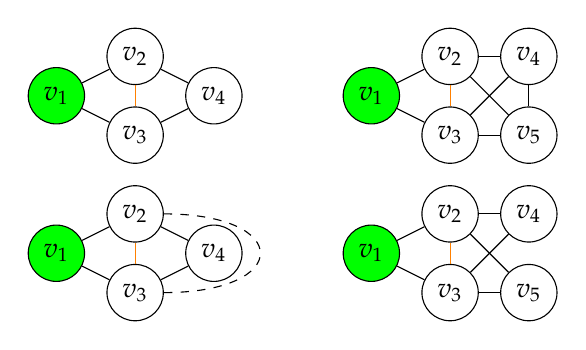
\begin{tikzpicture}
\begin{scope}[every node/.style={circle,draw}]               
	%k3+k3    
    \node[fill=green] (a) at (0,1) {$v_1$};
 	\node (b) at (1,1.5) {$v_2$};
 	\node (c) at (1,0.5) {$v_3$};
 	\node (d) at (2,1) {$v_4$};
    \path [-] (a) edge (b);
    \path [-] (a) edge (c);
    \draw[orange] (c) -- (b);        
    \path [-] (c) edge (d);
    \path [-] (b) edge (d);
    %k3+k4
    \node[fill=green] (aa) at (4,1) {$v_1$};
 	\node (bb) at (5,1.5) {$v_2$};
 	\node (cc) at (5,0.5) {$v_3$};
 	\node (dd) at (6,1.5) {$v_4$};
 	\node (ee) at (6, 0.5) {$v_5$};
    \path [-] (aa) edge (bb);
    \path [-] (aa) edge (cc);
    \draw[orange] (cc) -- (bb);        
    \path [-] (bb) edge (dd);
    \path [-] (cc) edge (ee);
    \path [-] (dd) edge (ee);
    \path [-] (dd) edge (cc);
    \path [-] (bb) edge (ee);   
    %k3+(k3+cm)
    \node[fill=green] (A) at (0,-1) {$v_1$};
 	\node (B) at (1,-0.5) {$v_2$};
 	\node (C) at (1,-1.5) {$v_3$};
 	\node (D) at (2,-1) {$v_4$};
    \path [-] (A) edge (B);
    \path [-] (A) edge (C);
    \draw[orange] (C) -- (B);     
    \path [-] (C) edge (D);
    \path [-] (B) edge (D);
    %k3+(k3+k3)
    \node[fill=green] (AA) at (4,-1) {$v_1$};
 	\node (BB) at (5,-0.5) {$v_2$};
 	\node (CC) at (5,-1.5) {$v_3$};
 	\node (DD) at (6,-0.5) {$v_4$};
 	\node (EE) at (6,-1.5) {$v_5$};
    \path [-] (AA) edge (BB);
    \path [-] (AA) edge (CC);
    \draw[orange] (CC) -- (BB);        
    \path [-] (CC) edge (DD);
    \path [-] (BB) edge (DD);
    \path [-] (BB) edge (EE);
    \path [-] (CC) edge (EE);        
    
\end{scope}
	\draw[dashed] (B) .. controls (3,-0.5) and (3,-1.5) .. (C);
\end{tikzpicture}
\caption{A simplicial $K_3$ over $\{v_1,v_2,v_3\}$ shares an edge with a $K_3$ (top left), $K_4$ (top right), $\{K_3, C_m\}$ (bottom left) or $\{K_3,K_3\}$ (bottom right).}
\label{fg:k3+}
\end{figure} 

\textbf{Lloyd's conjecture:} knowing a graph is WRS, adding an edge to obtain a supergraph, perhaps it is efficient to check if the supergraph is wrs.

\begin{proof}
because remove the added edge, then we obtain the original graph which we know is wrs. however, we don't remove a random edge when checking wrs unless the edge connects to a simplicial node. what if the edge is not connected with a sim node? if we know the original graph is wrs and we know the set of sim nodes in the recursion and the set of edges to delete, then we could easily check if the new edge is connected with any one of the sim node, if it is then good. if not, then we could check if the new edge is connected with two neighbours of a sim node, if it is then good. if a graph is wrs, then it eventually will diminish, so the new edge must appear somewhere in the recursion to either stop the recursion or don't stop it.
\end{proof} 

\begin{corollary}
DAGs in the same Markov equivalent class produce the same Markov blanket sets $B_X$. 
\end{corollary}
\begin{proof}
If two DAGs $G_1$ and $G_2$ are Markov equivalent, they have the same skeleton and the same set of colliders. This implies $B_i^{G_1} = B_i^{G_2}, \forall X_i \in X$. \qed
\end{proof}
Notice that two Markov equivalent classes could entail the same $B_X$. For example... 

\begin{corollary}
$|\{\text{chordal graphs}\}| \le |B_X| \le |\{\text{Markov equivalent classes}\}|$.
\end{corollary} 

Counting labelled chordal graphs \cite{wormald1985counting}, counting Markov equivalent classes (assymptotic ratio of around 0.27 to DAGs) \cite{gillispie2001enumerating}. 

\begin{table}[]
\centering
\caption{Comparison between the number of labelled connected chordal graphs, the number of weak recursively simplicial graphs, the number of undirected graphs and the number of Markov equivalent classes.}
\label{my-label}
\begin{tabular}{llllll}
\# nodes & \# con-C.G. & \# C.G. & \# WRS & \# U.G. & \# MEC \\ \hline
1        & 1& 1                 & 1          & 1         & 1 \\
2        & 1 & 2                 & 2          & 2         & 2 \\
3        & 4 & 8                 & 8          & 8         & 11 \\
4        & 35 & 61                & 61         & 64         & 185 \\
5        & 541 & 822               & 882        & 1024            & 8782\\
6        & 13302 & 18154             &       & 32768              & 1067825\\
7        & 489287 & 617675            &            & 2097152         & 312510571\\
8        & 25864897 & 30888596          &            &  268435456        & 212133402500 \\
9        & 1910753782 & 2192816760        &            &  68719476736       & 326266056291213 \\ 
10       & $1.93 \times 10^{11}$ & $2.15 \times 10^{11}$     &            & $3.52 \times 10^{13}$  & $1.19\times 10^{17}$ \\ \hline
\end{tabular}
\end{table}

\begin{proposition}
\label{prop:leaf_is_sim}
Let $G$ be a DAG and $F$ be the moral graph of $G$. If a node $x$ is a leaf in $G$, then it must be a simplicial node in $F$. 
\end{proposition}
\begin{proof}
If $x$ is a leaf in $G$, it has only parents, which form a clique after moralization. By definition, $x$ is a simplicial node in $F$. \qed
\end{proof}

\begin{corollary}
Let $G$ be a DAG and $F$ be the moral graph of $G$. Then $F$ must have at least one simplicial node. 
\end{corollary}

\begin{proof}
Since each DAG has at least one leaf, by Proposition \ref{prop:leaf_is_sim} $F$ have at least one simplicial node. \qed
\end{proof}

\begin{corollary}
\label{cor:negation_of_leaf_is_sim}
Let $G$ be a DAG and $F$ be the moral graph of $G$. If a node $x$ is not a simplicial node in $F$, then it must not be a leaf in $G$. 
\end{corollary}

\begin{proposition}
Let $G$ be a DAG and $F$ be the moral graph of $G$. Let $S^1$ be the set of simplicial nodes in $F$ and $F_1$ be the induced subgraph of $F$ over $X\setminus S^1$. Then there must exist at least one simplicial node after removing from $F'$ all the edges between $N(X_i), \forall X_i \in S^1$.
\end{proposition}

\begin{proof}
Let $F_1'$ be the result of removing from $F_1$ all the edges between $N(X_i), \forall X_i \in S^1$. The corresponding directed graph $G'$ of $F_1'$ must be a subgraph of the DAG $G$, so also acyclic. Assuming $F_1'$ has no simplicial nodes, by Corollary \ref{cor:negation_of_leaf_is_sim} $G'$ has no leaf, which is a contradiction. \qed
\end{proof}


Here are some issues worth discussing:
\begin{enumerate}
\item Application: the backtracking algorithm can now be applied when learning MBs in paralle. What if there are conflicts between two MBs, which one should give up? Need to estimate uncertainty?
\item Simplicial nodes in the first step always contain the leaves.
\item Those nodes that become simplicial in the next step without having to delete any edges contain the leaves in the next step. 
\item So wrs can be used to test if a MB family is consistent with a DAG, it would be good if we can also find out how many consistent DAGs or essential graphs are there for this MB family. 
\item also it would be good if we can explore wrs into details, such as what dag nodes become simplicial nodes in wrs recursion, and if no edges need to be deleted from a simplicial node's neighbours then what's this simplicial node?
\item maybe there is a path from s.t. every step is a moral graph of a dag, perhaps can be proved by delete an edge from a dag.   
\end{enumerate}

\textbf{Questions:} If a graph $F$ is known to be wrs, does is help to decide if a subgraph/supergraph different by one edge from $F$ is wrs or not?

\textbf{Answer:} Probably not. If it is, then we know a base case, any graph can be reached from this base case, hence any graph can be efficiently tested. 

\iffalse
The undirected edge connects two parents of a common child is called a \textit{moralized edge}. The process of obtaining a moral graph from a DAG is called \textit{moralization}. There is a unique moral graph of each DAG. Next, we define the reverse of a moralization process as \textit{demoralization}. It is defined on undirected graphs with at least one simplicial node. 
\fi

% the next proposition may not be true, so we omit it.
\iffalse
The next proposition proves that a chordal graph is also D-WRS, but not vice versa. 
\begin{proposition}
\label{prop:chordal_is_dwrs}
If $F=(V,E)$ is a chordal graph, then it is D-WRS. 
\end{proposition}
\begin{proof}
Assuming $F$ is not D-WRS. Then there is a subgraph $F' \subset F$ obtained by recursively remvoing all simplicial cliques from $F$ s.t. $F'$ has no simplicial clique. Hence, $F'$ must be cyclic 
\end{proof}


\begin{proof}
Being chordal is equivalent as being triangulated. If $F$ is chordal (Figure \ref{fg:chordal_is_dwrs}), removing the maximal simplicial clique of size 3 results in a subgraph of $F$ that has a maximal simplicial clique of size 2. Removing the size 2 maximal simplicial clique, we obtain a subgraph  that could also be obtained by recursively simplicial. \qed
\end{proof}
\begin{figure}[H]
\centering
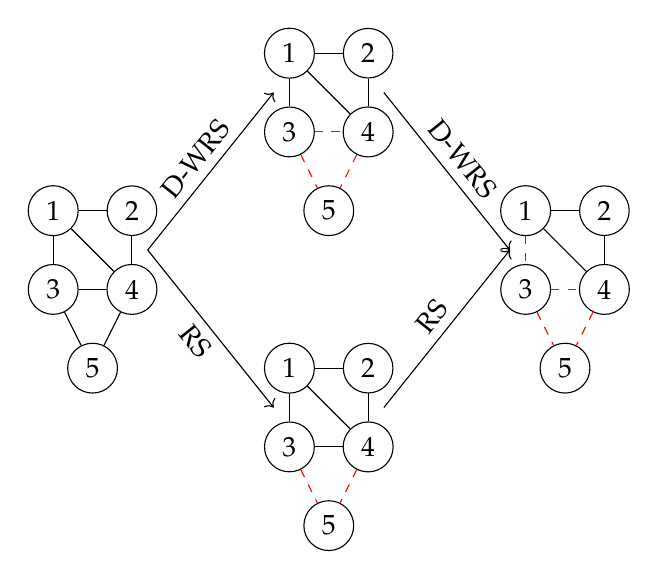
\begin{tikzpicture}
%\tikzstyle{place}=[circle,draw=blue!50,fill=blue!20,thick,inner sep=0pt,minimum size=6mm]
\begin{scope}[every node/.style={circle,draw}]  
    \node (F) at (0,0) {$1$};
    \node (G) at (1,0) {$2$};
    \node (H) at (0,-1) {$3$};
    \node (I) at (1,-1) {$4$};
    \node (J) at (0.5,-2) {$5$};
     
    \node (A) at (3,2) {$1$};
    \node (B) at (4,2) {$2$};
    \node (C) at (3,1) {$3$};
    \node (D) at (4,1) {$4$};
    \node (E) at (3.5,0) {$5$};
    
    \node (a) at (3,-2) {$1$};
    \node (b) at (4,-2) {$2$};
    \node (c) at (3,-3) {$3$};
    \node (d) at (4,-3) {$4$};
    \node (e) at (3.5,-4) {$5$};
    
    \node (K) at (6,0) {$1$};
    \node (L) at (7,0) {$2$};
    \node (M) at (6,-1) {$3$};
    \node (N) at (7,-1) {$4$};
    \node (O) at (6.5,-2) {$5$};
\end{scope}

\begin{scope}[>={Stealth[black]}]    
    \path [-] (F) edge (G);
    \path [-] (F) edge (H);
    \path [-] (G) edge (I);
    \path [-] (H) edge (I);
    \path [-] (H) edge (J);
    \path [-] (I) edge (J);
    \path [-] (F) edge (I);
        
    \path [-] (A) edge (B);
    \path [-] (A) edge (C);
    \path [-] (B) edge (D);
    \path [color=red,dashed] [-] (C) edge (D);
    \path [color=red,dashed][-] (C) edge (E);
    \path [color=red,dashed][-] (D) edge (E);
    \path [-] (A) edge (D);
    
    \path [-] (a) edge (b);
    \path [-] (a) edge (c);
    \path [-] (b) edge (d);
    \path [-] (c) edge (d);
    \path [color=red,dashed][-] (c) edge (e);
    \path [color=red,dashed][-] (d) edge (e);
    \path [-] (a) edge (d);
    
    \path [-] (K) edge (L);
    \path [color=red,dashed][-] (K) edge (M);
    \path [-] (L) edge (N);
    \path [color=red,dashed][-] (M) edge (N);
    \path [color=red,dashed][-] (M) edge (O);
    \path [color=red,dashed][-] (N) edge (O);
    \path [-] (K) edge (N);
\end{scope}

\begin{scope}[->,every node/.style={midway,sloped}]
	\draw (1.2,-0.5) -- (2.8,1.5) node[above] {D-WRS};
	\draw (1.2,-0.5) -- (2.8,-2.5) node[below] {RS};
    \draw (4.2,1.5) -- (5.8,-0.5) node[above] {D-WRS};
	\draw (4.2,-2.5) -- (5.8,-0.5) node[above] {RS};
\end{scope}	
\end{tikzpicture}
\caption{An example of a chordal graph is also D-WRS.}
\label{fg:chordal_is_dwrs}
\end{figure}

The converse of this proposition is not necessarily true (e.g., Figure \ref{fg:envelope}). If $F$ is a moral graph s.t. $\Delta(F) \le 2$, then F must be a tree hence chordal. By Proposition \ref{prop:chordal_is_dwrs} it must be D-WRS too. Next, we prove that $F$ is also D-WRS if $\Delta(F)=3$.
\fi

\section{Appendix}
\subsection{Reduction of 3-CNF to graph morality}
The following is the proof of Proposition \ref{prop:deg5} that states the problem of checking morality for maximum degree $5$ graphs is NP-complete. 
\begin{proof}
We use the same argument that \citeauthor{verma1993deciding} used. That is, present a polynomial time reduction from 3-CNF to graph morality. The nodes that have degree greater than $5$ in their construction are $\{v_i^{15},\bar{v}_i^{15}, S^7\}$ (\cite{verma1993deciding} Figure $4$), which have arbitrary high degrees depending on the number of clauses $t$ in a 3-CNF problem. To reduce their high degrees, we revise \citeauthor{verma1993deciding}'s construction based on the same variable gedget and clause gedget, but a different auxiliary gedget (Figure \ref{fg:variable_gedget}, \ref{fg:clause_gedget}, \ref{fg:aux_gedget} respectively) and different connection rules. 

The detailed construction rules are in \cite{verma1993deciding}. The high level description is that put the envelope graph in the auxiliary gedget at the top, so that it initializes downward directions. Since each gedget contains an envelope subgraph, it can be partially directed. The $K_4$ in each of the clause gedget ensures that network flow does not go through the envelop subgraph that corresponds to the negation of a variable in a variable gedget. The key differences between the revised construction and the original construction are as the following. The clause gedgets are connected by a chain to get rid of the high degree node that connects to all clause gedgets. Only the first two clause gedgets are connected to a variable gedget directly and hence form a $K_3$. For example, the $K_3$ formed by $\{F_2^1,F_3^1,\bar{X}^{15}\}$. Any additional clause gedget is connected to a variable gedget via the formed $K_3$, not directly onto the variable gedget. For example, node $F_4^1$ is connected to $F_3^1$ and hence $\{F_4^1,F_3^1,F_3^3\}$ form another $K_3$. The final constructed graph is shown in Figure \ref{fg:3cnf}. \qed
\end{proof}
\begin{figure}[H]
\centering
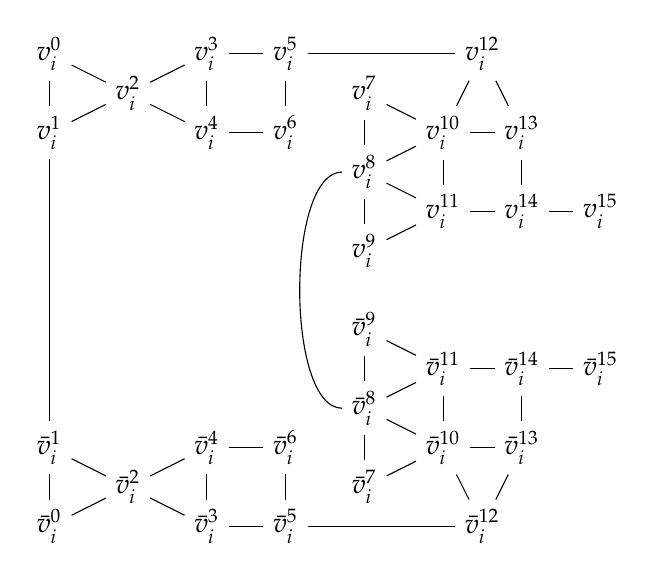
\begin{tikzpicture}
%\tikzstyle{place}=[circle,draw=blue!50,fill=blue!20,thick,inner sep=0pt,minimum size=6mm]
%\begin{scope}[every node/.style={circle,thick,draw,minimum size=3mm}]
\begin{scope}
    \node (A) at (0,3.5) {$v_i^0$};
    \node (B) at (0,2.5) {$v_i^1$};
    \node (C) at (1,3) {$v_i^2$};
    \node (D) at (2,3.5) {$v_i^3$};
    \node (E) at (2,2.5) {$v_i^4$};
    \node (F) at (3,3.5) {$v_i^5$};
    \node (G) at (3,2.5) {$v_i^6$};
    \node (H) at (4,3) {$v_i^7$};
    \node (I) at (4,2) {$v_i^8$};
    \node (J) at (4,1) {$v_i^9$};
    \node (K) at (5,2.5) {$v_i^{10}$};
    \node (L) at (5,1.5) {$v_i^{11}$};
    \node (M) at (5.5,3.5) {$v_i^{12}$};
    \node (N) at (6,2.5) {$v_i^{13}$};
    \node (O) at (6,1.5) {$v_i^{14}$};
    \node (P) at (7,1.5) {$v_i^{15}$};
    
    \node (a) at (0,-2.5) {$\bar{v}_i^0$};
    \node (b) at (0,-1.5) {$\bar{v}_i^1$};
    \node (c) at (1,-2) {$\bar{v}_i^2$};
    \node (d) at (2,-2.5) {$\bar{v}_i^3$};
    \node (e) at (2,-1.5) {$\bar{v}_i^4$};
    \node (f) at (3,-2.5) {$\bar{v}_i^5$};
    \node (g) at (3,-1.5) {$\bar{v}_i^6$};
    \node (h) at (4,-2) {$\bar{v}_i^7$};
    \node (i) at (4,-1) {$\bar{v}_i^8$};
    \node (j) at (4,0) {$\bar{v}_i^9$};
    \node (k) at (5,-1.5) {$\bar{v}_i^{10}$};
    \node (l) at (5,-0.5) {$\bar{v}_i^{11}$};
    \node (m) at (5.5,-2.5) {$\bar{v}_i^{12}$};
    \node (n) at (6,-1.5) {$\bar{v}_i^{13}$};
    \node (o) at (6,-0.5) {$\bar{v}_i^{14}$};
    \node (p) at (7,-0.5) {$\bar{v}_i^{15}$};
\end{scope}

\begin{scope}[>={Stealth[black]},
              every edge/.style={draw=black}]
    \path [-] (B) edge (b);
    \path [-] (A) edge (B);
    \path [-] (A) edge (C);
    \path [-] (B) edge (C);
    \path [-] (C) edge (D);
    \path [-] (C) edge (E);
    \path [-] (D) edge (E);
    \path [-] (D) edge (F);
    \path [-] (E) edge (G);
    \path [-] (F) edge (G);
    \path [-] (F) edge (M);
    \path [-] (H) edge (I);
    \path [-] (H) edge (K);
    \path [-] (K) edge (I);
    \path [-] (I) edge (J);
    \path [-] (I) edge (L);
    \path [-] (L) edge (J);
    \path [-] (K) edge (M);
    \path [-] (K) edge (N);
    \path [-] (K) edge (L);
    \path [-] (M) edge (N);
    \path [-] (N) edge (O);
    \path [-] (L) edge (O);
    \path [-] (O) edge (P);
    
    \path [-] (a) edge (b);
    \path [-] (a) edge (c);
    \path [-] (b) edge (c);
    \path [-] (c) edge (d);
    \path [-] (c) edge (e);
    \path [-] (d) edge (e);
    \path [-] (d) edge (f);
    \path [-] (e) edge (g);
    \path [-] (f) edge (g);
    \path [-] (f) edge (m);
    \path [-] (h) edge (i);
    \path [-] (h) edge (k);
    \path [-] (k) edge (i);
    \path [-] (i) edge (j);
    \path [-] (i) edge (l);
    \path [-] (l) edge (j);
    \path [-] (k) edge (m);
    \path [-] (k) edge (n);
    \path [-] (k) edge (l);
    \path [-] (m) edge (n);
    \path [-] (n) edge (o);
    \path [-] (l) edge (o);
    \path [-] (o) edge (p);
    
    %\path [-] (I) edge (i);
\end{scope}
\draw[-] (I) .. controls (3,2) and (3,-1) .. (i);
\end{tikzpicture}
\caption{A variable gedget for $v_i$. It contains $32$ nodes, where the top half corresponding to the variable and the bottom half corresponding to the negation of the variable.}
\label{fg:variable_gedget}
\end{figure}

\begin{figure}[H]
\centering
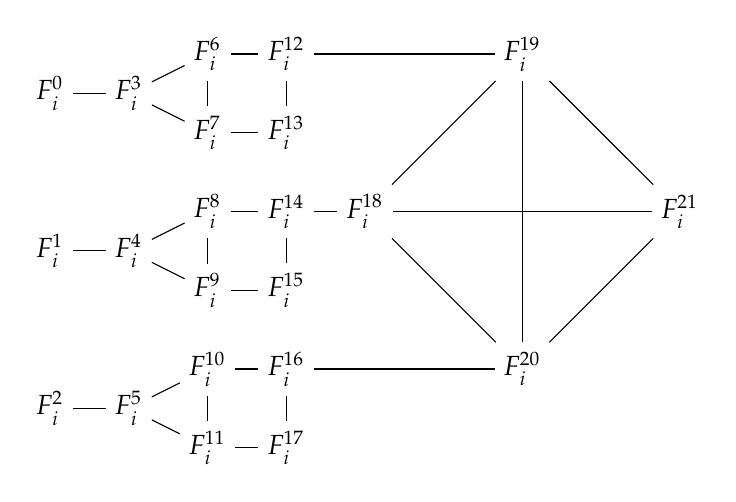
\begin{tikzpicture}
%\tikzstyle{place}=[circle,draw=blue!50,fill=blue!20,thick,inner sep=0pt,minimum size=6mm]
%\begin{scope}[every node/.style={circle,thick,draw,minimum size=3mm}]
\begin{scope}
    \node (a) at (0,4.5) {$F_i^0$};
    \node (b) at (0,2.5) {$F_i^1$};   
    \node (c) at (0,0.5) {$F_i^2$};
    \node (d) at (1,4.5) {$F_i^3$};
    \node (e) at (1,2.5) {$F_i^4$};
    \node (f) at (1,0.5) {$F_i^5$};
    \node (g) at (2,5) {$F_i^6$};
    \node (h) at (2,4) {$F_i^7$};
    \node (i) at (2,3) {$F_i^8$};
    \node (j) at (2,2) {$F_i^9$};
    \node (k) at (2,1) {$F_i^{10}$};
    \node (l) at (2,0) {$F_i^{11}$};
    \node (m) at (3,5) {$F_i^{12}$};
    \node (n) at (3,4) {$F_i^{13}$};
    \node (o) at (3,3) {$F_i^{14}$};
    \node (p) at (3,2) {$F_i^{15}$};
    \node (q) at (3,1) {$F_i^{16}$};
    \node (r) at (3,0) {$F_i^{17}$};
    \node (s) at (4,3) {$F_i^{18}$};
    \node (t) at (6,5) {$F_i^{19}$};
    \node (u) at (6,1) {$F_i^{20}$};
    \node (v) at (8,3) {$F_i^{21}$};
\end{scope}

\begin{scope}[>={Stealth[black]},every edge/.style={draw=black}]
    \path [-] (a) edge (d);
    \path [-] (d) edge (g);
    \path [-] (d) edge (h);
    \path [-] (g) edge (h);
    \path [-] (g) edge (m);
    \path [-] (h) edge (n);
    \path [-] (m) edge (n);
    \path [-] (m) edge (t);
    
    \path [-] (b) edge (e);
    \path [-] (i) edge (e);
    \path [-] (j) edge (e);
    \path [-] (i) edge (j);
    \path [-] (i) edge (o);
    \path [-] (j) edge (p);
    \path [-] (o) edge (p);
    \path [-] (o) edge (s);
    \path [-] (s) edge (u);
    \path [-] (s) edge (v);
    \path [-] (v) edge (u);
    \path [-] (t) edge (u);
    \path [-] (t) edge (v);
    \path [-] (t) edge (s);
    
    \path [-] (c) edge (f);
    \path [-] (f) edge (k);
    \path [-] (f) edge (l);
    \path [-] (k) edge (l);
    \path [-] (k) edge (q);
    \path [-] (l) edge (r);
    \path [-] (q) edge (r);
    \path [-] (q) edge (u);
\end{scope}
\end{tikzpicture}
\caption{A clause gedget for $F_i$. It contains $22$ nodes. Each of the three identical subgraphs corresponding to a variable in the clause $F_i$.}
\label{fg:clause_gedget}
\end{figure}

\begin{figure}[H]
\centering
\begin{tikzpicture}
\begin{scope}
    \node (a) at (1,4.5) {$S^0$};
    \node (b) at (2,5) {$S^1$};   
    \node (c) at (2,4) {$S^2$};
    \node (d) at (3,5) {$S^3$};
    \node (e) at (3,4) {$S^4$};
    
    \node (f) at (1,3) {$S^5$};
    \node (g) at (2,3) {$S^6$};
    \node (h) at (3,3) {$S^7_1$};
    \node (i) at (6,3) {$S^7_t$};
    
    \path [-] (a) edge (b);
    \path [-] (a) edge (c);
    \path [-] (b) edge (c);
    \path [-] (b) edge (d);
    \path [-] (c) edge (e);
    \path [-] (d) edge (e);
    \path [-] (f) edge (g);
	\path [-] (h) edge (g);
	\path [-] (h) edge (3.5,3);
	\path [-] (5.5,3) edge (i);
	\path [densely dashed] (4,3) edge (5,3);
\end{scope}
\end{tikzpicture}
\caption{An auxiliary gedget that contains $7+t$ nodes, where $t$ is the number of clauses in the 3-CNF.}
\label{fg:aux_gedget}
\end{figure}

\begin{figure}[H]
\centering
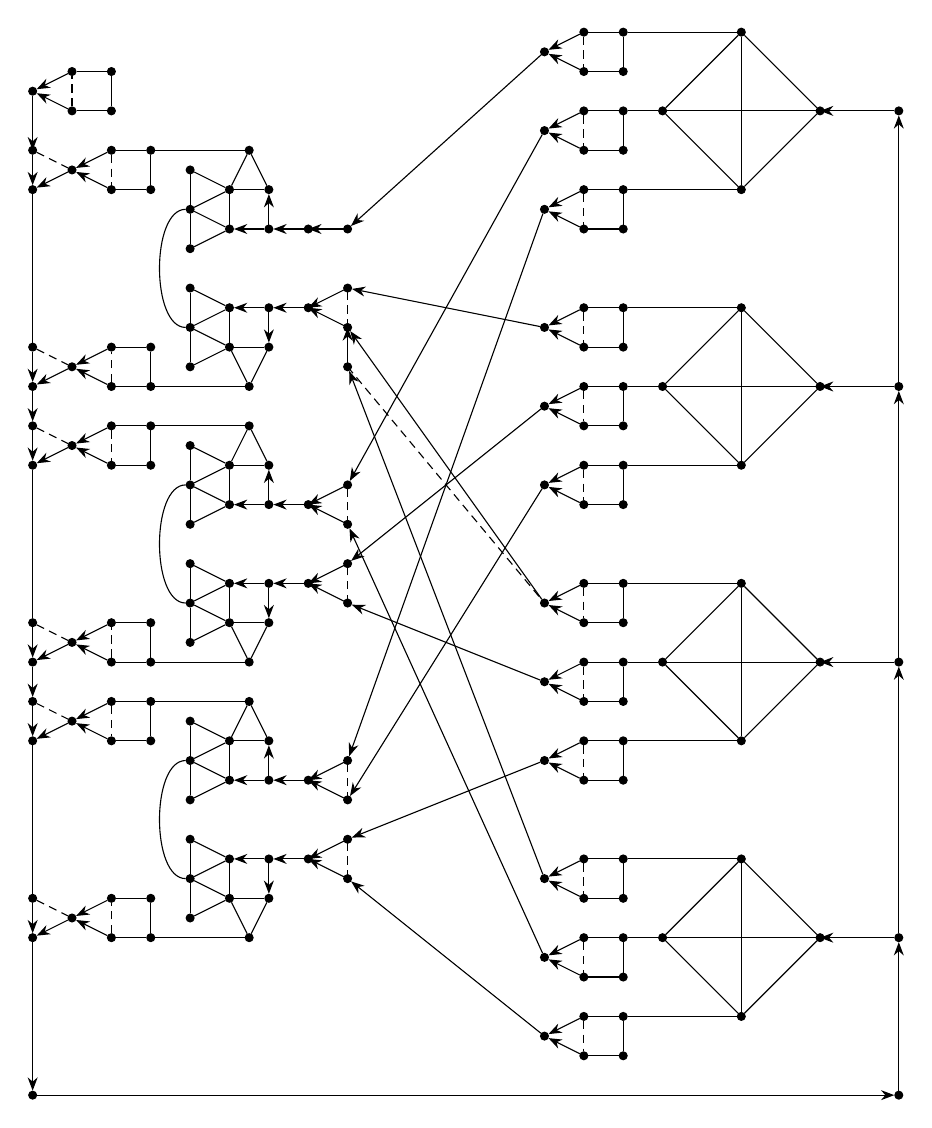
\begin{tikzpicture}
% variable gedget
\begin{scope}[every node/.style={circle,draw,fill=black,minimum size=1mm,inner sep=1pt},>={Stealth[black]}]
    \node (A) at (0,0.5) {};
    \node (B) at (0,1) {};
    \node (C) at (0.5,0.75) {};
    \node (D) at (1,0.5) {};
    \node (E) at (1,1) {};
    \node (F) at (1.5,0.5) {};
    \node (G) at (1.5,1) {};
    \node (H) at (2,0.75) {};
    \node (I) at (2,1.25) {};
    \node (J) at (2,1.75) {};
    \node (K) at (2.5,1) {};
    \node (L) at (2.5,1.5) {};
    \node (M) at (2.75,0.5) {};
    \node (N) at (3,1) {};
    \node (O) at (3,1.5) {};
    \node (P) at (3.5,1.5) {};
    \node (a) at (0,3.5) {};
    \node (b) at (0,3) {};
    \node (c) at (0.5,3.25) {};
    \node (d) at (1,3.5) {};
    \node (e) at (1,3) {};
    \node (f) at (1.5,3.5) {};
    \node (g) at (1.5,3) {};
    \node (h) at (2,3.25) {};
    \node (i) at (2,2.75) {};
    \node (j) at (2,2.25) {};
    \node (k) at (2.5,3) {};
    \node (l) at (2.5,2.5) {};
    \node (m) at (2.75,3.5) {};
    \node (n) at (3,3) {};
    \node (o) at (3,2.5) {};
    \node (p) at (3.5,2.5) {};
    
    \node (A1) at (0,0.5+3.5) {};
    \node (B1) at (0,1+3.5) {};
    \node (C1) at (0.5,0.75+3.5) {};
    \node (D1) at (1,0.5+3.5) {};
    \node (E1) at (1,1+3.5) {};
    \node (F1) at (1.5,0.5+3.5) {};
    \node (G1) at (1.5,1+3.5) {};
    \node (H1) at (2,0.75+3.5) {};
    \node (I1) at (2,1.25+3.5) {};
    \node (J1) at (2,1.75+3.5) {};
    \node (K1) at (2.5,1+3.5) {};
    \node (L1) at (2.5,1.5+3.5) {};
    \node (M1) at (2.75,0.5+3.5) {};
    \node (N1) at (3,1+3.5) {};
    \node (O1) at (3,1.5+3.5) {};
    \node (P1) at (3.5,1.5+3.5) {};
    \node (a1) at (0,3.5+3.5) {};
    \node (b1) at (0,3+3.5) {};
    \node (c1) at (0.5,3.25+3.5) {};
    \node (d1) at (1,3.5+3.5) {};
    \node (e1) at (1,3+3.5) {};
    \node (f1) at (1.5,3.5+3.5) {};
    \node (g1) at (1.5,3+3.5) {};
    \node (h1) at (2,3.25+3.5) {};
    \node (i1) at (2,2.75+3.5) {};
    \node (j1) at (2,2.25+3.5) {};
    \node (k1) at (2.5,3+3.5) {};
    \node (l1) at (2.5,2.5+3.5) {};
    \node (m1) at (2.75,3.5+3.5) {};
    \node (n1) at (3,3+3.5) {};
    \node (o1) at (3,2.5+3.5) {};
    \node (p1) at (3.5,2.5+3.5) {};
    
    \node (A2) at (0,0.5+7) {};
    \node (B2) at (0,1+7) {};
    \node (C2) at (0.5,0.75+7) {};
    \node (D2) at (1,0.5+7) {};
    \node (E2) at (1,1+7) {};
    \node (F2) at (1.5,0.5+7) {};
    \node (G2) at (1.5,1+7) {};
    \node (H2) at (2,0.75+7) {};
    \node (I2) at (2,1.25+7) {};
    \node (J2) at (2,1.75+7) {};
    \node (K2) at (2.5,1+7) {};
    \node (L2) at (2.5,1.5+7) {};
    \node (M2) at (2.75,0.5+7) {};
    \node (N2) at (3,1+7) {};
    \node (O2) at (3,1.5+7) {};
    \node (P2) at (3.5,1.5+7) {};
    \node (a2) at (0,3.5+7) {};
    \node (b2) at (0,3+7) {};
    \node (c2) at (0.5,3.25+7) {};
    \node (d2) at (1,3.5+7) {};
    \node (e2) at (1,3+7) {};
    \node (f2) at (1.5,3.5+7) {};
    \node (g2) at (1.5,3+7) {};
    \node (h2) at (2,3.25+7) {};
    \node (i2) at (2,2.75+7) {};
    \node (j2) at (2,2.25+7) {};
    \node (k2) at (2.5,3+7) {};
    \node (l2) at (2.5,2.5+7) {};
    \node (m2) at (2.75,3.5+7) {};
    \node (n2) at (3,3+7) {};
    \node (o2) at (3,2.5+7) {};
    \node (p2) at (3.5,2.5+7) {};

    \path [-] (B) edge (b);
    \path [->] (B) edge (A);
    \path [->] (C) edge (A);
    \path [densely dashed] (B) edge (C);
    \path [->] (D) edge (C);
    \path [->] (E) edge (C);
    \path [densely dashed] (D) edge (E);
    \path [-] (D) edge (F);
    \path [-] (E) edge (G);
    \path [-] (F) edge (G);
    \path [-] (F) edge (M);
    \path [-] (H) edge (I);
    \path [-] (H) edge (K);
    \path [-] (K) edge (I);
    \path [-] (I) edge (J);
    \path [-] (I) edge (L);
    \path [-] (L) edge (J);
    \path [-] (K) edge (M);
    \path [-] (K) edge (N);
    \path [-] (K) edge (L);
    \path [-] (M) edge (N);
    \path [->] (O) edge (N);
    \path [->] (O) edge (L);
    \path [->] (P) edge (O);
    \path [->] (a) edge (b);
    \path [densely dashed] (a) edge (c);
    \path [->] (c) edge (b);
    \path [->] (d) edge (c);
    \path [->] (e) edge (c);
    \path [densely dashed] (d) edge (e);
    \path [-] (d) edge (f);
    \path [-] (e) edge (g);
    \path [-] (f) edge (g);
    \path [-] (f) edge (m);
    \path [-] (h) edge (i);
    \path [-] (h) edge (k);
    \path [-] (k) edge (i);
    \path [-] (i) edge (j);
    \path [-] (i) edge (l);
    \path [-] (l) edge (j);
    \path [-] (k) edge (m);
    \path [-] (k) edge (n);
    \path [-] (k) edge (l);
    \path [-] (m) edge (n);
    \path [->] (o) edge (n);
    \path [->] (o) edge (l);
    \path [->] (p) edge (o);
    \draw[-] (I) .. controls (1.5,1.25) and (1.5,2.75) .. (i);
    
    \path [-] (B1) edge (b1);
    \path [->] (B1) edge (A1);
    \path [->] (C1) edge (A1);
    \path [densely dashed] (B1) edge (C1);
    \path [->] (D1) edge (C1);
    \path [->] (E1) edge (C1);
    \path [densely dashed] (D1) edge (E1);
    \path [-] (D1) edge (F1);
    \path [-] (E1) edge (G1);
    \path [-] (F1) edge (G1);
    \path [-] (F1) edge (M1);
    \path [-] (H1) edge (I1);
    \path [-] (H1) edge (K1);
    \path [-] (K1) edge (I1);
    \path [-] (I1) edge (J1);
    \path [-] (I1) edge (L1);
    \path [-] (L1) edge (J1);
    \path [-] (K1) edge (M1);
    \path [-] (K1) edge (N1);
    \path [-] (K1) edge (L1);
    \path [-] (M1) edge (N1);
    \path [->] (O1) edge (N1);
    \path [->] (O1) edge (L1);
    \path [->] (P1) edge (O1);
    \path [->] (a1) edge (b1);
    \path [densely dashed] (a1) edge (c1);
    \path [->] (c1) edge (b1);
    \path [->] (d1) edge (c1);
    \path [->] (e1) edge (c1);
    \path [densely dashed] (d1) edge (e1);
    \path [-] (d1) edge (f1);
    \path [-] (e1) edge (g1);
    \path [-] (f1) edge (g1);
    \path [-] (f1) edge (m1);
    \path [-] (h1) edge (i1);
    \path [-] (h1) edge (k1);
    \path [-] (k1) edge (i1);
    \path [-] (i1) edge (j1);
    \path [-] (i1) edge (l1);
    \path [-] (l1) edge (j1);
    \path [-] (k1) edge (m1);
    \path [-] (k1) edge (n1);
    \path [-] (k1) edge (l1);
    \path [-] (m1) edge (n1);
    \path [->] (o1) edge (n1);
    \path [->] (o1) edge (l1);
    \path [->] (p1) edge (o1);
    \draw[-] (I1) .. controls (1.5,1.25+3.5) and (1.5,2.75+3.5) .. (i1);
    
    \path [-] (B2) edge (b2);
    \path [->] (B2) edge (A2);
    \path [->] (C2) edge (A2);
    \path [densely dashed] (B2) edge (C2);
    \path [->] (D2) edge (C2);
    \path [->] (E2) edge (C2);
    \path [densely dashed] (D2) edge (E2);
    \path [-] (D2) edge (F2);
    \path [-] (E2) edge (G2);
    \path [-] (F2) edge (G2);
    \path [-] (F2) edge (M2);
    \path [-] (H2) edge (I2);
    \path [-] (H2) edge (K2);
    \path [-] (K2) edge (I2);
    \path [-] (I2) edge (J2);
    \path [-] (I2) edge (L2);
    \path [-] (L2) edge (J2);
    \path [-] (K2) edge (M2);
    \path [-] (K2) edge (N2);
    \path [-] (K2) edge (L2);
    \path [-] (M2) edge (N2);
    \path [->] (O2) edge (N2);
    \path [->] (O2) edge (L2);
    \path [->] (P2) edge (O2);
    \path [->] (a2) edge (b2);
    \path [densely dashed] (a2) edge (c2);
    \path [->] (c2) edge (b2);
    \path [->] (d2) edge (c2);
    \path [->] (e2) edge (c2);
    \path [densely dashed] (d2) edge (e2);
    \path [-] (d2) edge (f2);
    \path [-] (e2) edge (g2);
    \path [-] (f2) edge (g2);
    \path [-] (f2) edge (m2);
    \path [-] (h2) edge (i2);
    \path [-] (h2) edge (k2);
    \path [-] (k2) edge (i2);
    \path [-] (i2) edge (j2);
    \path [-] (i2) edge (l2);
    \path [-] (l2) edge (j2);
    \path [-] (k2) edge (m2);
    \path [-] (k2) edge (n2);
    \path [-] (k2) edge (l2);
    \path [-] (m2) edge (n2);
    \path [->] (o2) edge (n2);
    \path [->] (o2) edge (l2);
    \path [->] (p2) edge (o2);
    \draw[-] (I2) .. controls (1.5,1.25+7) and (1.5,2.75+7) .. (i2);
    
    \path [->] (A1) edge (a);
    \path [->] (A2) edge (a1);
\end{scope}

% clause gedget >={Stealth[black]},every node/.style={fill=white,circle},
\begin{scope}[every node/.style={circle,draw,fill=black,minimum size=1mm,inner sep=1pt},>={Stealth[black]}]
    \node (a) at (4,7.75) {};
    \path [->] (4,7.75) edge (4,8.25);
    \draw[densely dashed] (4,7.75) edge (6.5,4.75);
    \node (b) at (4,5.75) {};  
    \path [->] (4,5.75) edge (3.5,6); 
    \draw[densely dashed] (4,5.75) edge (4,6.25);
    \node (c) at (4,1.25) {};
    \path [->] (4,1.25) edge (3.5,1.5);
    \draw[densely dashed] (4,1.25) edge (4,1.75);
    \node (d) at (0+6.5,2.25-1) {};
    \node (e) at (0+6.5,1.25-1) {};
    \node (f) at (0+6.5,0.25-1) {};
    \node (g) at (0.5+6.5,2.5-1) {};
    \node (h) at (0.5+6.5,2-1) {};
    \node (i) at (0.5+6.5,1.5-1) {};
    \node (j) at (0.5+6.5,1-1) {};
    \node (k) at (0.5+6.5,0.5-1) {};
    \node (l) at (0.5+6.5,0-1) {};
    \node (m) at (1+6.5,2.5-1) {};
    \node (n) at (1+6.5,2-1) {};
    \node (o) at (1+6.5,1.5-1) {};
    \node (p) at (1+6.5,1-1) {};
    \node (q) at (1+6.5,0.5-1) {};
    \node (r) at (1+6.5,0-1) {};
    \node (s) at (1.5+6.5,1.5-1) {};
    \node (t) at (2.5+6.5,2.5-1) {};
    \node (u) at (2.5+6.5,0.5-1) {};
    \node (v) at (3.5+6.5,1.5-1) {};
    \path [<-] (a) edge (d);
    \path [<-] (d) edge (g);
    \path [<-] (d) edge (h);
    \path [densely dashed] (g) edge (h);
    \path [-] (g) edge (m);
    \path [-] (h) edge (n);
    \path [-] (m) edge (n);
    \path [-] (m) edge (t);
    \path [<-] (b) edge (e);
    \path [->] (i) edge (e);
    \path [->] (j) edge (e);
    \path [densely dashed] (i) edge (j);
    \path [-] (i) edge (o);
    \path [-] (j) edge (p);
    \path [-] (o) edge (p);
    \path [-] (o) edge (s);
    \path [-] (s) edge (u);
    \path [-] (s) edge (v);
    \path [-] (v) edge (u);
    \path [-] (t) edge (u);
    \path [-] (t) edge (v);
    \path [-] (t) edge (s);
    \path [<-] (c) edge (f);
    \path [<-] (f) edge (k);
    \path [<-] (f) edge (l);
    \path [densely dashed] (k) edge (l);
    \path [-] (k) edge (q);
    \path [-] (l) edge (r);
    \path [-] (q) edge (r);
    \path [-] (q) edge (u);
    
    \node (a1) at (4,8.25) {};
    \path [->] (4,8.25) edge (3.5,8.5);
    \draw[densely dashed] (4,8.25) edge (4,8.75);
    \node (b1) at (4,4.75) {};   
    \path [->] (4,4.75) edge (3.5,5);
    \draw[densely dashed] (4,4.75) edge (4,5.25);
    \node (c1) at (4,1.75) {};
    \path [->] (4,1.75) edge (3.5,1.5);
    \node (d1) at (0+6.5,2.25-1+3.5) {};
    \node (e1) at (0+6.5,1.25-1+3.5) {};
    \node (f1) at (0+6.5,0.25-1+3.5) {};
    \node (g1) at (0.5+6.5,2.5-1+3.5) {};
    \node (h1) at (0.5+6.5,2-1+3.5) {};
    \node (i1) at (0.5+6.5,1.5-1+3.5) {};
    \node (j1) at (0.5+6.5,1-1+3.5) {};
    \node (k1) at (0.5+6.5,0.5-1+3.5) {};
    \node (l1) at (0.5+6.5,0-1+3.5) {};
    \node (m1) at (1+6.5,2.5-1+3.5) {};
    \node (n1) at (1+6.5,2-1+3.5) {};
    \node (o1) at (1+6.5,1.5-1+3.5) {};
    \node (p1) at (1+6.5,1-1+3.5) {};
    \node (q1) at (1+6.5,0.5-1+3.5) {};
    \node (r1) at (1+6.5,0-1+3.5) {};
    \node (s1) at (1.5+6.5,1.5-1+3.5) {};
    \node (t1) at (2.5+6.5,2.5-1+3.5) {};
    \node (u1) at (2.5+6.5,0.5-1+3.5) {};
    \node (v1) at (3.5+6.5,1.5-1+3.5) {};
    \path [<-] (a1) edge (d1);
    \path [<-] (d1) edge (g1);
    \path [<-] (d1) edge (h1);
    \path [densely dashed] (g1) edge (h1);
    \path [-] (g1) edge (m1);
    \path [-] (h1) edge (n1);
    \path [-] (m1) edge (n1);
    \path [-] (m1) edge (t1);
    \path [<-] (b1) edge (e1);
    \path [->] (i1) edge (e1);
    \path [->] (j1) edge (e1);
    \path [densely dashed] (i1) edge (j1);
    \path [-] (i1) edge (o1);
    \path [-] (j1) edge (p1);
    \path [-] (o1) edge (p1);
    \path [-] (o1) edge (s1);
    \path [-] (s1) edge (u1);
    \path [-] (s1) edge (v1);
    \path [-] (v1) edge (u1);
    \path [-] (t1) edge (u1);
    \path [-] (t1) edge (v1);
    \path [-] (t1) edge (s1);
    \path [<-] (c1) edge (f1);
    \path [<-] (f1) edge (k1);
    \path [<-] (f1) edge (l1);
    \path [densely dashed] (k1) edge (l1);
    \path [-] (k1) edge (q1);
    \path [-] (l1) edge (r1);
    \path [-] (q1) edge (r1);
    \path [-] (q1) edge (u1);
    
    \node (a2) at (4,8.75) {};
    \path [->] (4,8.75) edge (3.5,8.5);
    \node (b2) at (4,5.25) {};   
    \path [->] (4,5.25) edge (3.5,5);
    \node (c2) at (4,2.25) {};
    \path [->] (4,2.25) edge (3.5,2.5);
    \draw[densely dashed] (4,2.25) edge (4,2.75);
    \node (d2) at (0+6.5,2.25-1+7) {};
    \node (e2) at (0+6.5,1.25-1+7) {};
    \node (f2) at (0+6.5,0.25-1+7) {};
    \node (g2) at (0.5+6.5,2.5-1+7) {};
    \node (h2) at (0.5+6.5,2-1+7) {};
    \node (i2) at (0.5+6.5,1.5-1+7) {};
    \node (j2) at (0.5+6.5,1-1+7) {};
    \node (k2) at (0.5+6.5,0.5-1+7) {};
    \node (l2) at (0.5+6.5,0-1+7) {};
    \node (m2) at (1+6.5,2.5-1+7) {};
    \node (n2) at (1+6.5,2-1+7) {};
    \node (o2) at (1+6.5,1.5-1+7) {};
    \node (p2) at (1+6.5,1-1+7) {};
    \node (q2) at (1+6.5,0.5-1+7) {};
    \node (r2) at (1+6.5,0-1+7) {};
    \node (s2) at (1.5+6.5,1.5-1+7) {};
    \node (t2) at (2.5+6.5,2.5-1+7) {};
    \node (u2) at (2.5+6.5,0.5-1+7) {};
    \node (v2) at (3.5+6.5,1.5-1+7) {};
    \path [<-] (a2) edge (d2);
    \path [<-] (d2) edge (g2);
    \path [<-] (d2) edge (h2);
    \path [densely dashed] (g2) edge (h2);
    \path [-] (g2) edge (m2);
    \path [-] (h2) edge (n2);
    \path [-] (m2) edge (n2);
    \path [-] (m2) edge (t2);
    \path [<-] (b2) edge (e2);
    \path [->] (i2) edge (e2);
    \path [->] (j2) edge (e2);
    \path [densely dashed] (i2) edge (j2);
    \path [-] (i2) edge (o2);
    \path [-] (j2) edge (p2);
    \path [-] (o2) edge (p2);
    \path [-] (o2) edge (s2);
    \path [-] (s2) edge (u2);
    \path [-] (s2) edge (v2);
    \path [-] (v2) edge (u2);
    \path [-] (t2) edge (u2);
    \path [-] (t2) edge (v2);
    \path [-] (t2) edge (s2);
    \path [<-] (c2) edge (f2);
    \path [<-] (f2) edge (k2);
    \path [<-] (f2) edge (l2);
    \path [densely dashed] (k2) edge (l2);
    \path [-] (k2) edge (q2);
    \path [-] (l2) edge (r2);
    \path [-] (q2) edge (r2);
    \path [-] (q2) edge (u2);
    
    \node (a4) at (4,9.5) {};
    \path [->] (4,9.5) edge (3.5,9.5);
    \node (b4) at (4,6.25) {};   
    \path [->] (4,6.25) edge (3.5,6);
    \node (c4) at (4,2.75) {};
    \path [->] (4,2.75) edge (3.5,2.5);
    \node (d4) at (0+6.5,2.25-1+10.5) {};
    \node (e4) at (0+6.5,1.25-1+10.5) {};
    \node (f4) at (0+6.5,0.25-1+10.5) {};
    \node (g4) at (0.5+6.5,2.5-1+10.5) {};
    \node (h4) at (0.5+6.5,2-1+10.5) {};
    \node (i4) at (0.5+6.5,1.5-1+10.5) {};
    \node (j4) at (0.5+6.5,1-1+10.5) {};
    \node (k4) at (0.5+6.5,0.5-1+10.5) {};
    \node (l4) at (0.5+6.5,0-1+10.5) {};
    \node (m4) at (1+6.5,2.5-1+10.5) {};
    \node (n4) at (1+6.5,2-1+10.5) {};
    \node (o4) at (1+6.5,1.5-1+10.5) {};
    \node (p4) at (1+6.5,1-1+10.5) {};
    \node (q4) at (1+6.5,0.5-1+10.5) {};
    \node (r4) at (1+6.5,0-1+10.5) {};
    \node (s4) at (1.5+6.5,1.5-1+10.5) {};
    \node (t4) at (2.5+6.5,2.5-1+10.5) {};
    \node (u4) at (2.5+6.5,0.5-1+10.5) {};
    \node (v4) at (3.5+6.5,1.5-1+10.5) {};
    \path [<-] (a4) edge (d4);
    \path [<-] (d4) edge (g4);
    \path [<-] (d4) edge (h4);
    \path [densely dashed] (g4) edge (h4);
    \path [-] (g4) edge (m4);
    \path [-] (h4) edge (n4);
    \path [-] (m4) edge (n4);
    \path [-] (m4) edge (t4);
    \path [<-] (b4) edge (e4);
    \path [->] (i4) edge (e4);
    \path [->] (j4) edge (e4);
    \path [densely dashed] (i4) edge (j4);
    \path [-] (i4) edge (o4);
    \path [-] (j4) edge (p4);
    \path [-] (o4) edge (p4);
    \path [-] (o4) edge (s4);
    \path [-] (s4) edge (u4);
    \path [-] (s4) edge (v4);
    \path [-] (v4) edge (u4);
    \path [-] (t4) edge (u4);
    \path [-] (t4) edge (v4);
    \path [-] (t4) edge (s4);
    \path [<-] (c4) edge (f4);
    \path [<-] (f4) edge (k4);
    \path [<-] (f4) edge (l4);
    \path [densely dashed] (k4) edge (l4);
    \path [-] (k4) edge (q4);
    \path [-] (l4) edge (r4);
    \path [-] (q4) edge (r4);
    \path [-] (q4) edge (u4);
\end{scope}

% auxiliary gedget
\begin{scope}[every node/.style={circle,draw,fill=black,minimum size=1mm,inner sep=1pt},>={Stealth[black]}]
    \node (a) at (0,11.25) {};
    \node (b) at (0.5,11.5) {};
    \node (c) at (0.5,11) {};
    \node (d) at (1,11.5) {};
    \node (e) at (1,11) {};
    \path [<-] (a) edge (b);
    \path [<-] (a) edge (c);
    \path [densely dashed] (c) edge (b);
    \path [-] (d) edge (b);
    \path [-] (c) edge (e);
    \path [-] (d) edge (e);
    \path [->] (a) edge (0,10.5);
    
    \node (f) at (0,-1.5) {};
    \path[->] (0,0.5) edge (f);
    
    \node (g) at (11,-1.5) {};
    \node (h) at (11,0.5) {};
    \node (i) at (11,4) {};
    \node (j) at (11,7.5) {};
    \node (k) at (11,11) {};                
    \path [->] (f) edge (g);
    \path [->] (g) edge (h);
    \path [->] (h) edge (i);
    \path [->] (i) edge (j);
    \path [->] (j) edge (k);
    \path [->] (h) edge (10,0.5);
    \path [->] (i) edge (10,4);
    \path [->] (j) edge (10,7.5);
    \path [->] (k) edge (10,11);
\end{scope}
\end{tikzpicture}
\caption{A polynomial time construction that reduces 3-CNF to graph morality. The 3-CNF problem is $(X \vee Y \vee Z)\wedge(\bar{X} \vee \bar{Y} \vee Z)\wedge(\bar{X} \vee \bar{Y} \vee \bar{Z})\wedge(\bar{X} \vee Y \vee \bar{Z})$, where $X=1$ and $Y=Z=0$. This construction ensures that the resulting graph has maximum degree no more than $5$.}
\label{fg:3cnf}
\end{figure}


\subsection{Notations}
\begin{table}[]
\centering
\caption{Notations}
\label{my-label}
\begin{tabular}{ll}
\hline
$F$ &  a undirected graph \\
$G$ & a DAG \\
$X$ & a set of random variables (nodes) \\
$X_i$ & a random variable (or node) in $X$ \\
$X_{-i}$ & $X \setminus X_i$ \\ 
$X_{-[1,\dots, i]}$ & $X \setminus \{X_1, \dots, X_i\}$ \\ 
$B_i^G$ & the Markov blanket of a variable $X_i$ in $G$ \\ 
$B_X^G$ & $\{B_i \mid \forall X_i \in X\}$ \\ \hline
\end{tabular}
\end{table}

\bibliographystyle{named}
\bibliography{/home/kl/Documents/causal_discovery_ref_list}

\end{document}